\documentclass[8pt]{beamer}
\usepackage[absolute,overlay]{textpos}
%\documentclass[handout]{beamer}
%\usepackage{pgfpages}
%\pgfpagesuselayout{2 on 1}[a4paper,border shrink=5mm]
\usetheme{simple}

\usepackage{lmodern}
\usepackage[scale=2]{ccicons}

\usepackage{animate}

%quatation
\usepackage[style=british]{csquotes}
\def\signed #1{{\leavevmode\unskip\nobreak\hfil\penalty50\hskip1em
			\hbox{}\nobreak\hfill #1%
			\parfillskip=0pt \finalhyphendemerits=0 \endgraf}}
	
	\newsavebox\mybox
	\newenvironment{aquote}[1]
	{\savebox\mybox{#1}\begin{quote}\openautoquote\hspace*{-.7ex}}
		{\unskip\closeautoquote\vspace*{1mm}\signed{\usebox\mybox}\end{quote}}
	
%change font size
\newcommand\Fontvi{\fontsize{6}{7.2}\selectfont}

%change block params

	
% TODO: 
%   position adjustement
%   change colours
%       

% Watermark background (simple theme)

%\setwatermark{
\includegraphics[height=8cm]{./img/Heckert_GNU_white.png}}
\setwatermark{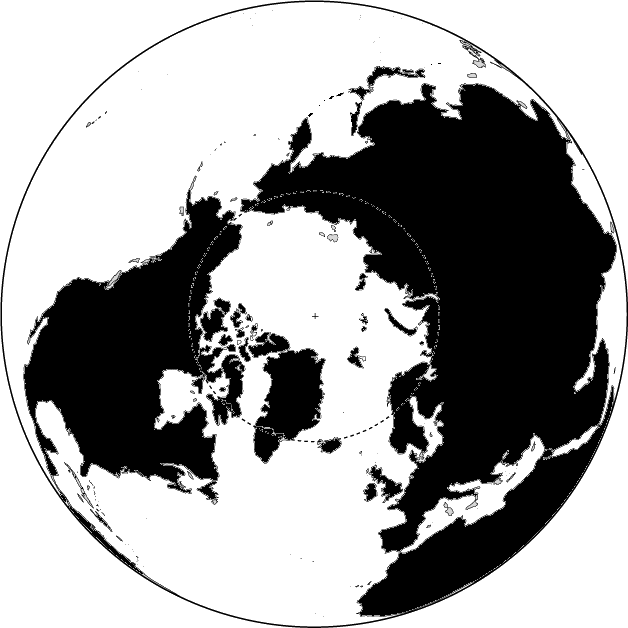
\includegraphics[height=8cm]{./img/arctic_transparent.png}}

\title{Laptev Sea and East Siberian Sea landfast ice: Mechanism of formation and variability of extent}
\date{\today}
\author{Valeria Selyuzhenok\\~\\\textsf {Approved Dissertation Committee}\\
	\textsf{Prof. Dr. R"udiger Gerdes}\\ 
	\textsf{Prof. Dr. Joachim Vogt}\\ 	
	\textsf{Dr. Thomas Krumpen}\\ }
\institute{Jacobs University Bremen}


\begin{document}
\maketitle
\logo[left]{
\includegraphics[height=0.5cm]{./img/logos.pdf}}
%\begin{flushright}
%		\textsf {Approved Dissertation Committee}\\[0.4cm]	
%		\textsf{Prof. Dr. R"udiger Gerdes}\\ 
%		\textsf{Prof. Dr. Joachim Vogt}\\ 	
%		\textsf{Dr. Thomas Krumpen}\\ 
%\end{flushright}
	
%slide 2
\setwatermark{\fontsize{125pt}{125pt}\selectfont{}}
\begin{frame}{Outline}
	\begin{columns}
	  \column{.8\textwidth}
		\begin{block}{I. Introduction}
		\end{block}
		\begin{block}{II. Variability of landfast ice extent and interannual changes}
		\end{block}
		\begin{block}{III. Mechanism of landfast ice development}
		\end{block}
		\begin{block}{IV. Summary and outlook} 
		\end{block}
	\end{columns}
\end{frame}

%slide 3
\setwatermark{\fontsize{125pt}{125pt}\selectfont{}}
\begin{frame}[fragile]{I. Arctic sea ice}
	\begin{columns}
		\column{0.5\textwidth}
			\begin{center}
				\textbf{17 March 2015}
			\end{center}
			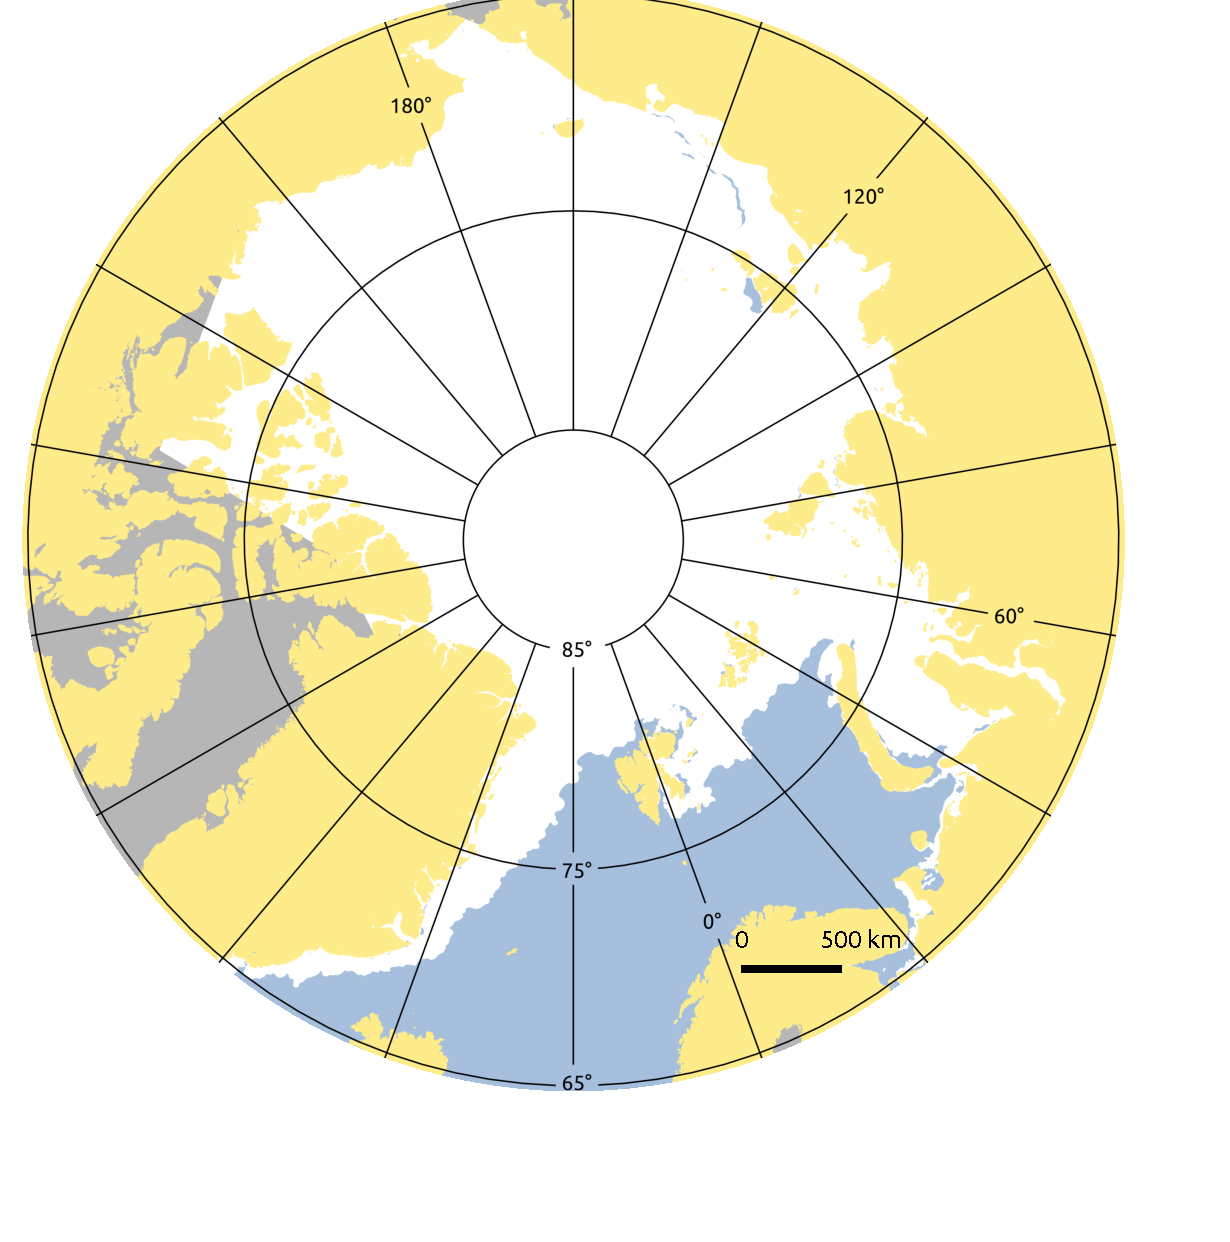
\includegraphics[width=1\textwidth]{./img/ArcticSI_Mar2015_SI_noLeg.pdf}\\
			
		\column{0.5\textwidth}
		\begin{center}
			\textbf{10 September 2015}
		\end{center}
			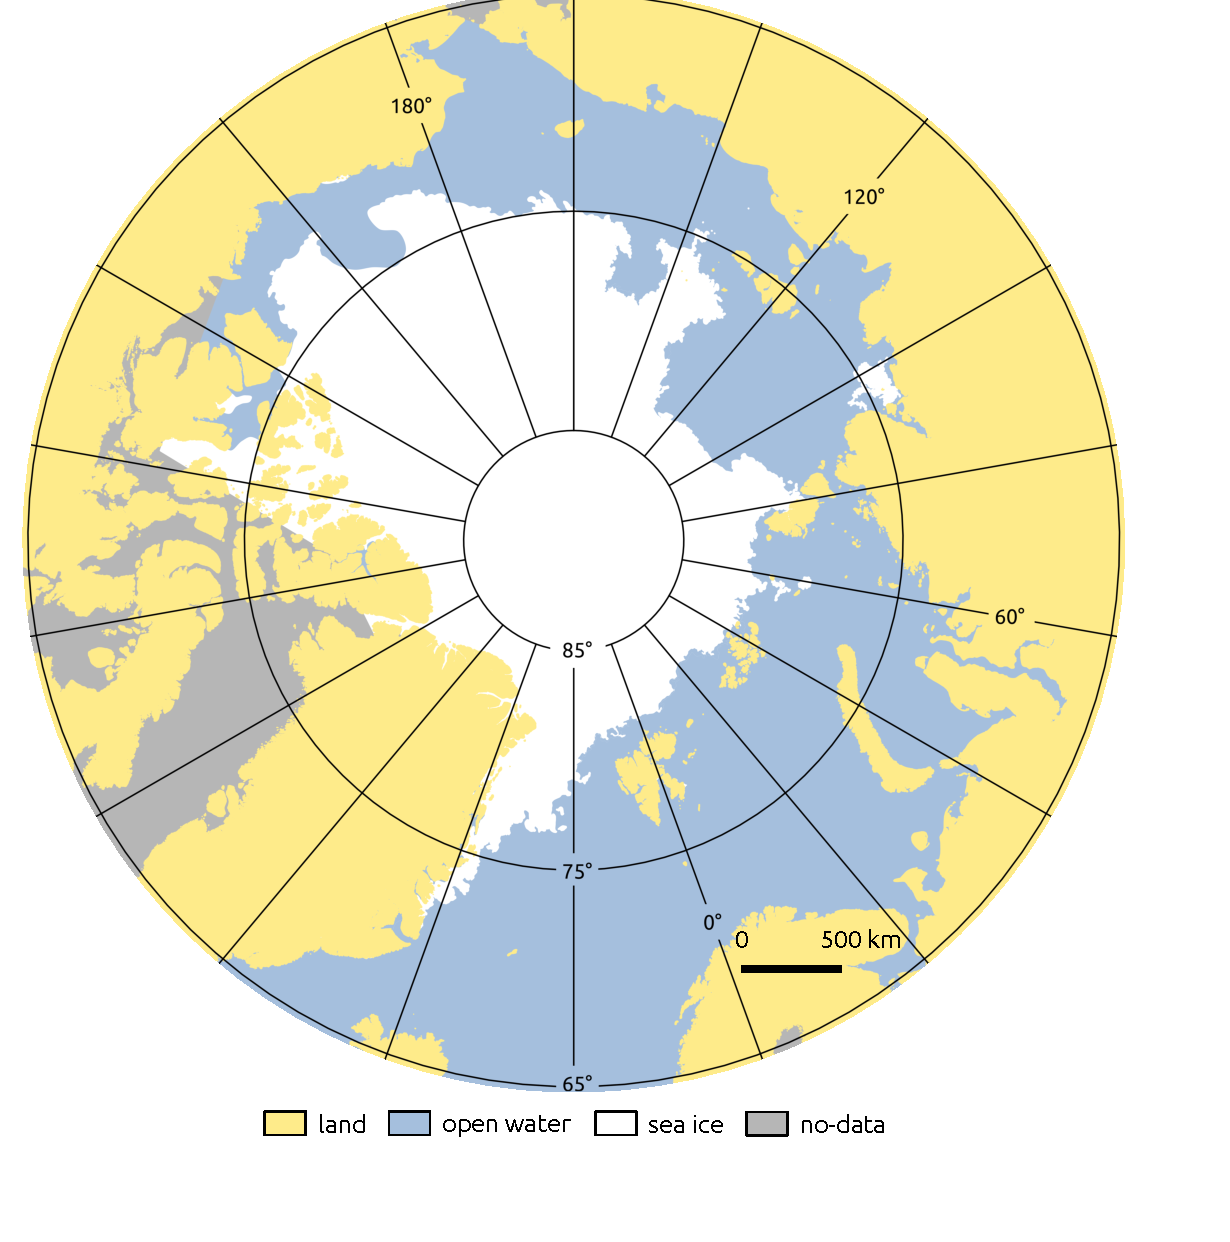
\includegraphics[width=1\textwidth]{./img/ArcticSI_Sep2015_crop.pdf}\\
	\end{columns}
\Fontvi
based on Operational Sea Ice Charts,\\
Arctic and Antarctic Research Institute, Russia (\textbf{AARI Charts})	
\end{frame}
	
%slide 4
\setwatermark{\fontsize{125pt}{125pt}\selectfont{}}
\begin{frame}[fragile]{I. The importance of Arctic sea ice}
	\begin{columns}
		\column[]{0.6\textwidth}
			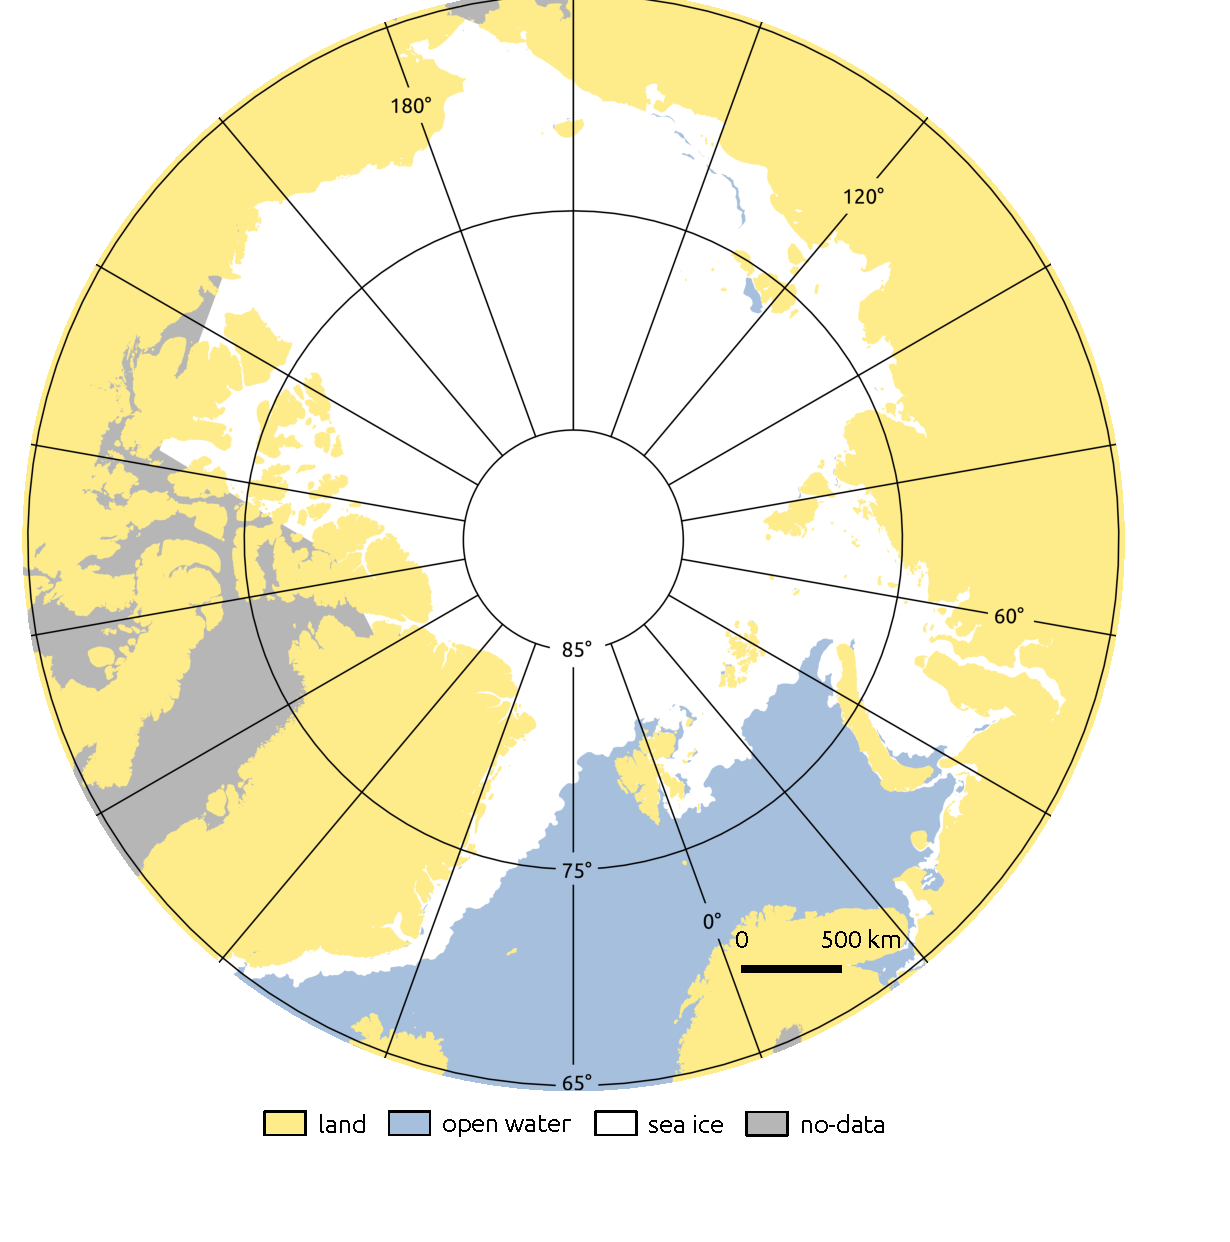
\includegraphics[width=1\textwidth]{./img/ArcticSI_Mar2015_SI.pdf}\\
		\column[]{0.4\textwidth}
	\begin{itemize}
		\item \textbf{Climate system:}\\ reflects about 80$\%$ of solar radiation\\~\\
		\item \textbf{Ecosystem:}\\ provides habitat and hunting platform\\~\\
		\item \textbf{Human activity:}\\ navigation, exploration, indigenous people activity
	\end{itemize}
	\end{columns}
\Fontvi
17 March 2015 (AARI Charts)
\end{frame}

%%slide 5
\setwatermark{\fontsize{125pt}{125pt}\selectfont{}}
\begin{frame}[fragile]{I. Arctic fast ice}
	\begin{columns}
		\column[]{0.6\textwidth}
		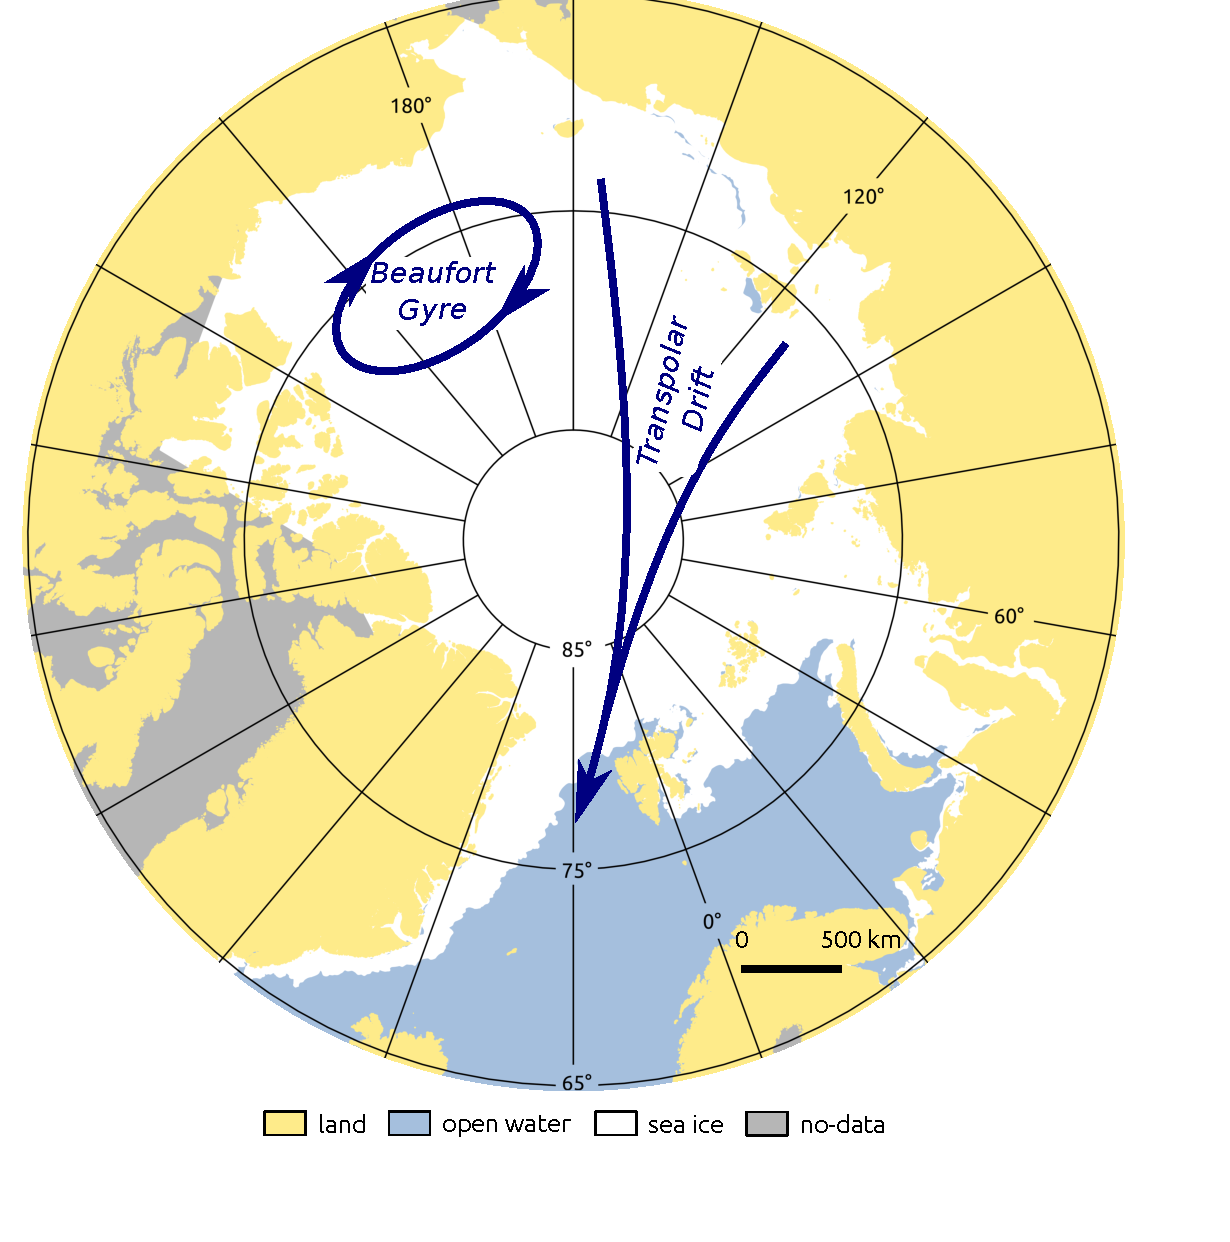
\includegraphics[width=1\textwidth]{./img/ArcticSI_Mar2015_SI_circ.pdf}\\
		\column[]{0.4\textwidth}
%		\begin{itemize}
%			\item \textbf{Climate system:}\\ reflects about 80$\%$ of solar radiation\\~\\
%			\item \textbf{Ecosystem:}\\ provides habitat and hunting platform\\~\\
%			\item \textbf{Human activity:}\\ navigation, exploration, indigenous people activity
%		\end{itemize}
	\end{columns}
\Fontvi
17 March 2015 (AARI Charts)
\end{frame}

%%slide 6
\setwatermark{\fontsize{125pt}{125pt}\selectfont{}}
\begin{frame}[fragile]{I. Arctic fast ice}
	\begin{columns}
		\column[]{0.5\textwidth}
		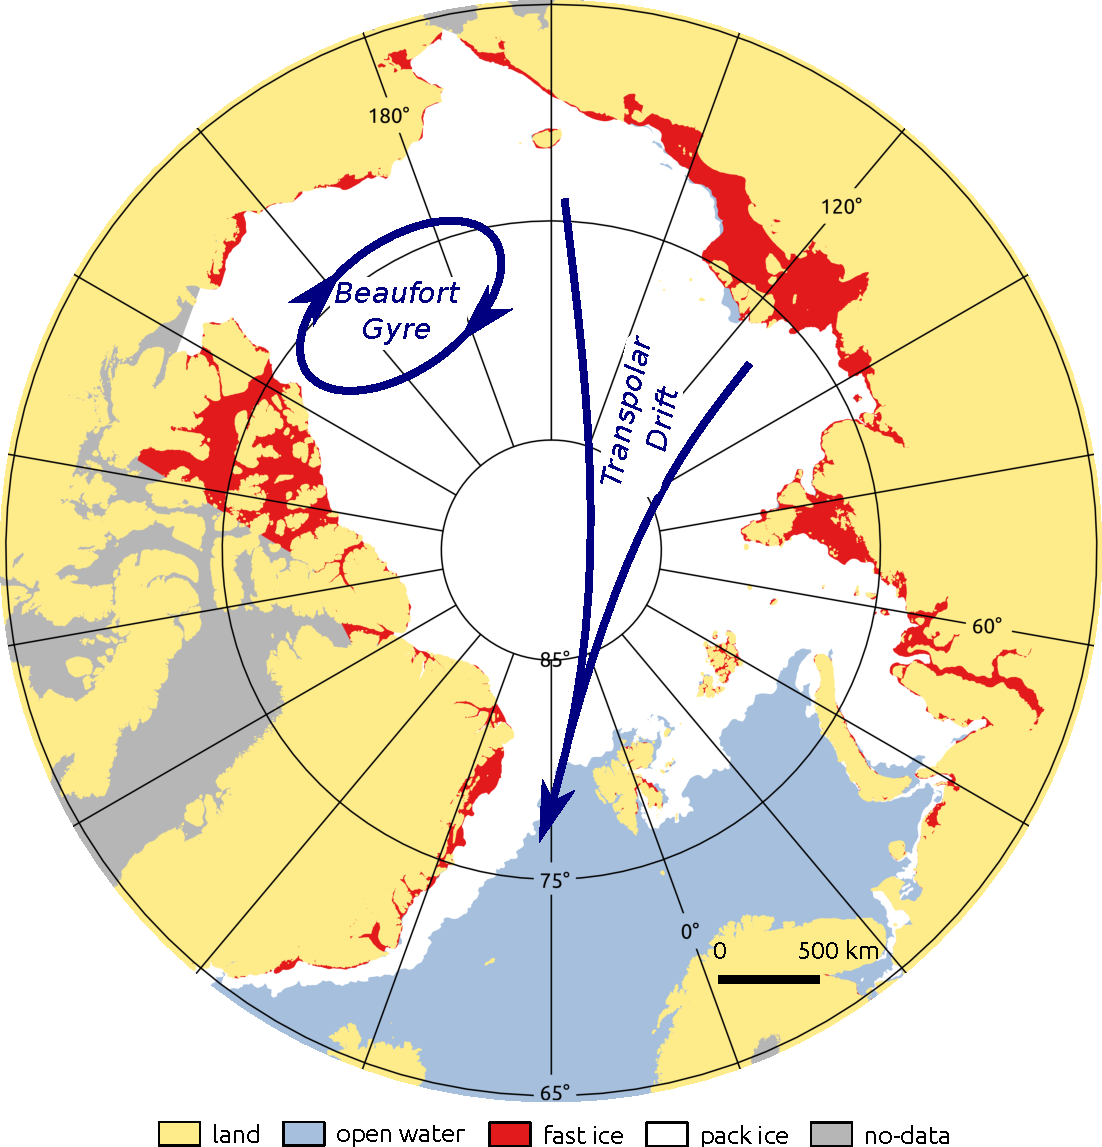
\includegraphics[width=1\textwidth]{./img/ArcticSI_Mar2015_circ.pdf}\\
		\column[]{0.5\textwidth}
				\begin{block}{\centering Definition}
					\centering
				Motionless and adjustent to the shore\\~\\
					\begin{itemize}
						\item \textbf{Operational charts} - experts opinion\\
						 (2-7 days, e.g. AARI charts)\\~\\
						\item \textbf{Remote sensing techniques}\\ - time interval between images\\
						 (e.g. 25 days - Mahoney et al. 2005)
					\end{itemize}
				\end{block}
				\begin{block}{\centering}
					\begin{center}
					 \textbf{$\sim$ 13$\%$ of total sea ice extent}
					\end{center}
				\end{block}
	\end{columns}
~\\
\Fontvi
17 March 2015 (AARI Charts)
\end{frame}


%slide 7
\setwatermark{\fontsize{125pt}{125pt}\selectfont{}}
\begin{frame}[fragile]{I.Importance of Arctic fast ice}
	\begin{columns}
		\column{0.5\textwidth}
			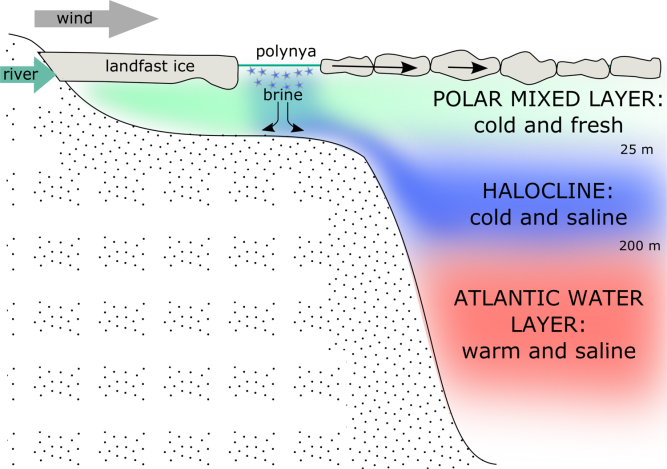
\includegraphics[width=1\textwidth]{./img/ImportanceFI.png}\\
		\column{0.5\textwidth}
		\begin{itemize}
			\item affects state of the Arctic Ocean and atmosphere\\(Maqueda et al. 2004, Itkin et al. 2015)\\~\\ 
			\item protects coasts from erosion\\(Rachold et al. 2000, Eicken et al. 2005)\\~\\ 
			\item helps to maintain submarine permafrost\\ (Rachold et al. 2000)\\~\\
			\item affects human activity\\(Johannessen et al. 2005, Hughes et al. 2011, Weintrit 2013)
		\end{itemize}
	\end{columns}
\Fontvi
Itkin et al. 2015
\end{frame}


%%slide 11
%\setwatermark{\fontsize{125pt}{125pt}\selectfont{}}
%\begin{frame}[fragile]{I. Changes in Arctic Sea ice}
%	\begin{columns}
%		\column{0.45\textwidth}
%		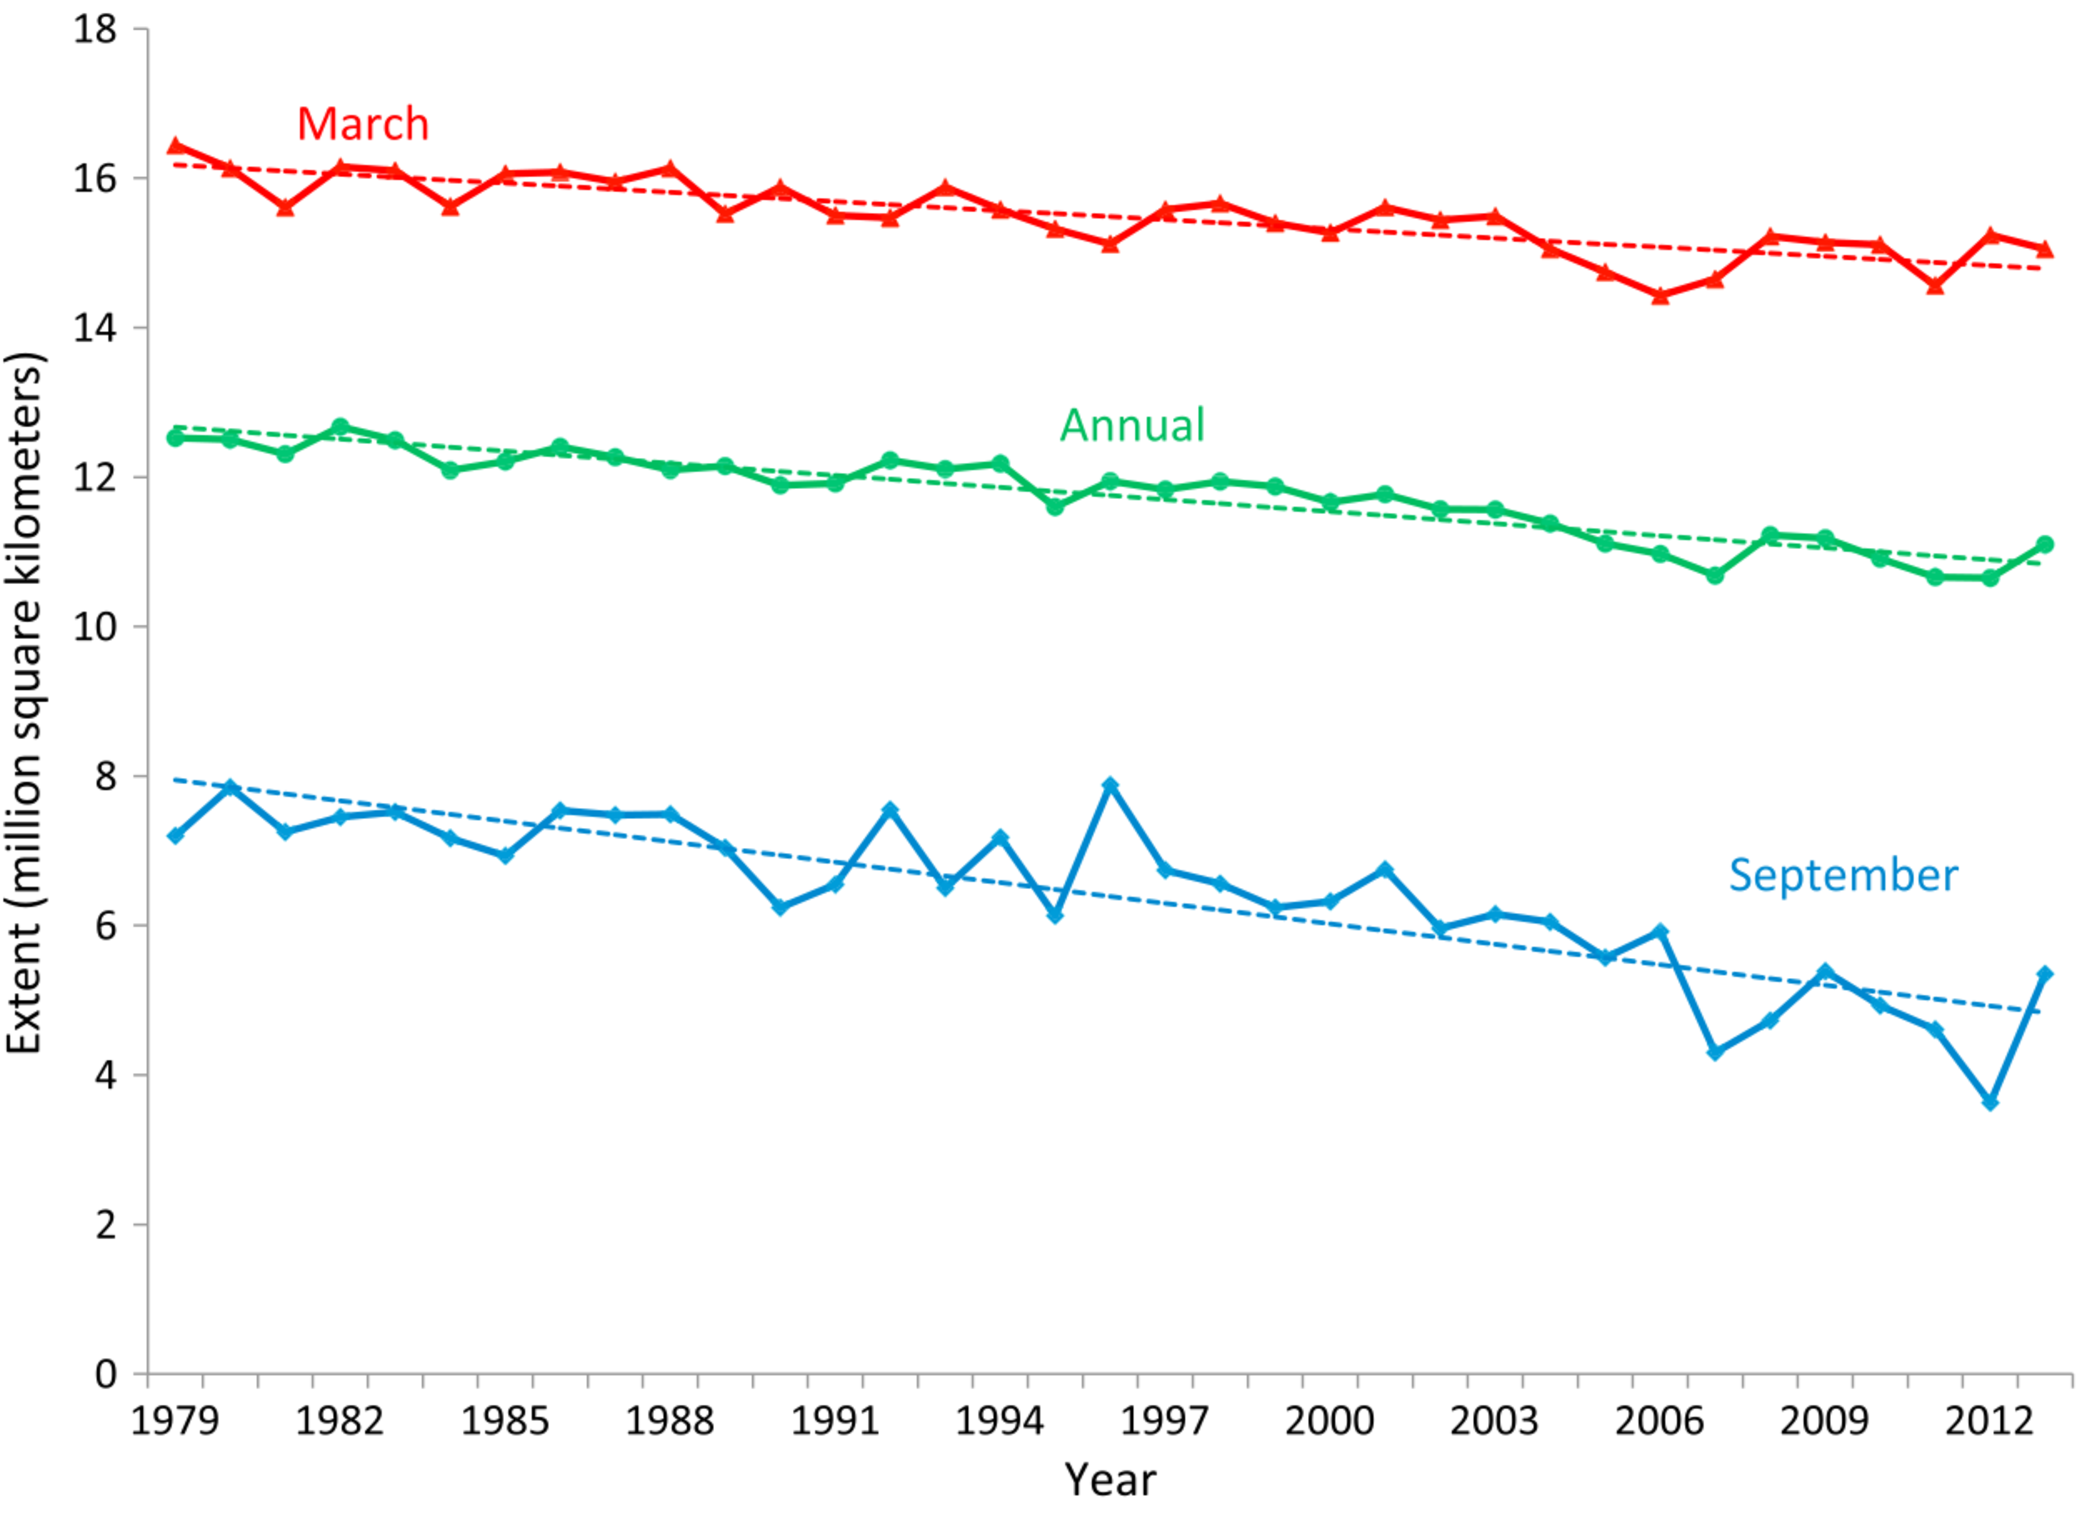
\includegraphics[height=5cm]{./img/Extent_trend.pdf}\\
%			\begin{center}
%			Monthly average total extent\\
%			\end{center}
%			\Fontvi
%			Meier et al.(2014)
%		\column{0.1\textwidth}
%		\column{0.4\textwidth}
%		\begin{itemize}
%			\item decrease in sea ice extent\\~\\
%			\item thinning of sea ice\\~\\
%			\item higher domination of younger ice types\\~\\
%		\end{itemize}
%
%	\end{columns}
%\end{frame}

%slide 8
\setwatermark{\fontsize{125pt}{125pt}\selectfont{}}
\begin{frame}[fragile]{I. Changes in Arctic fast ice, 1976-2007}
		\begin{columns}
			\column{0.5\textwidth}
			Changes in fast ice extent\\
			
			\column{0.5\textwidth}
			Long-term variation of fast ice extent\\ for the Northern Hemisphere\\

		\end{columns}
	\begin{columns}
		\column{0.5\textwidth}
		
		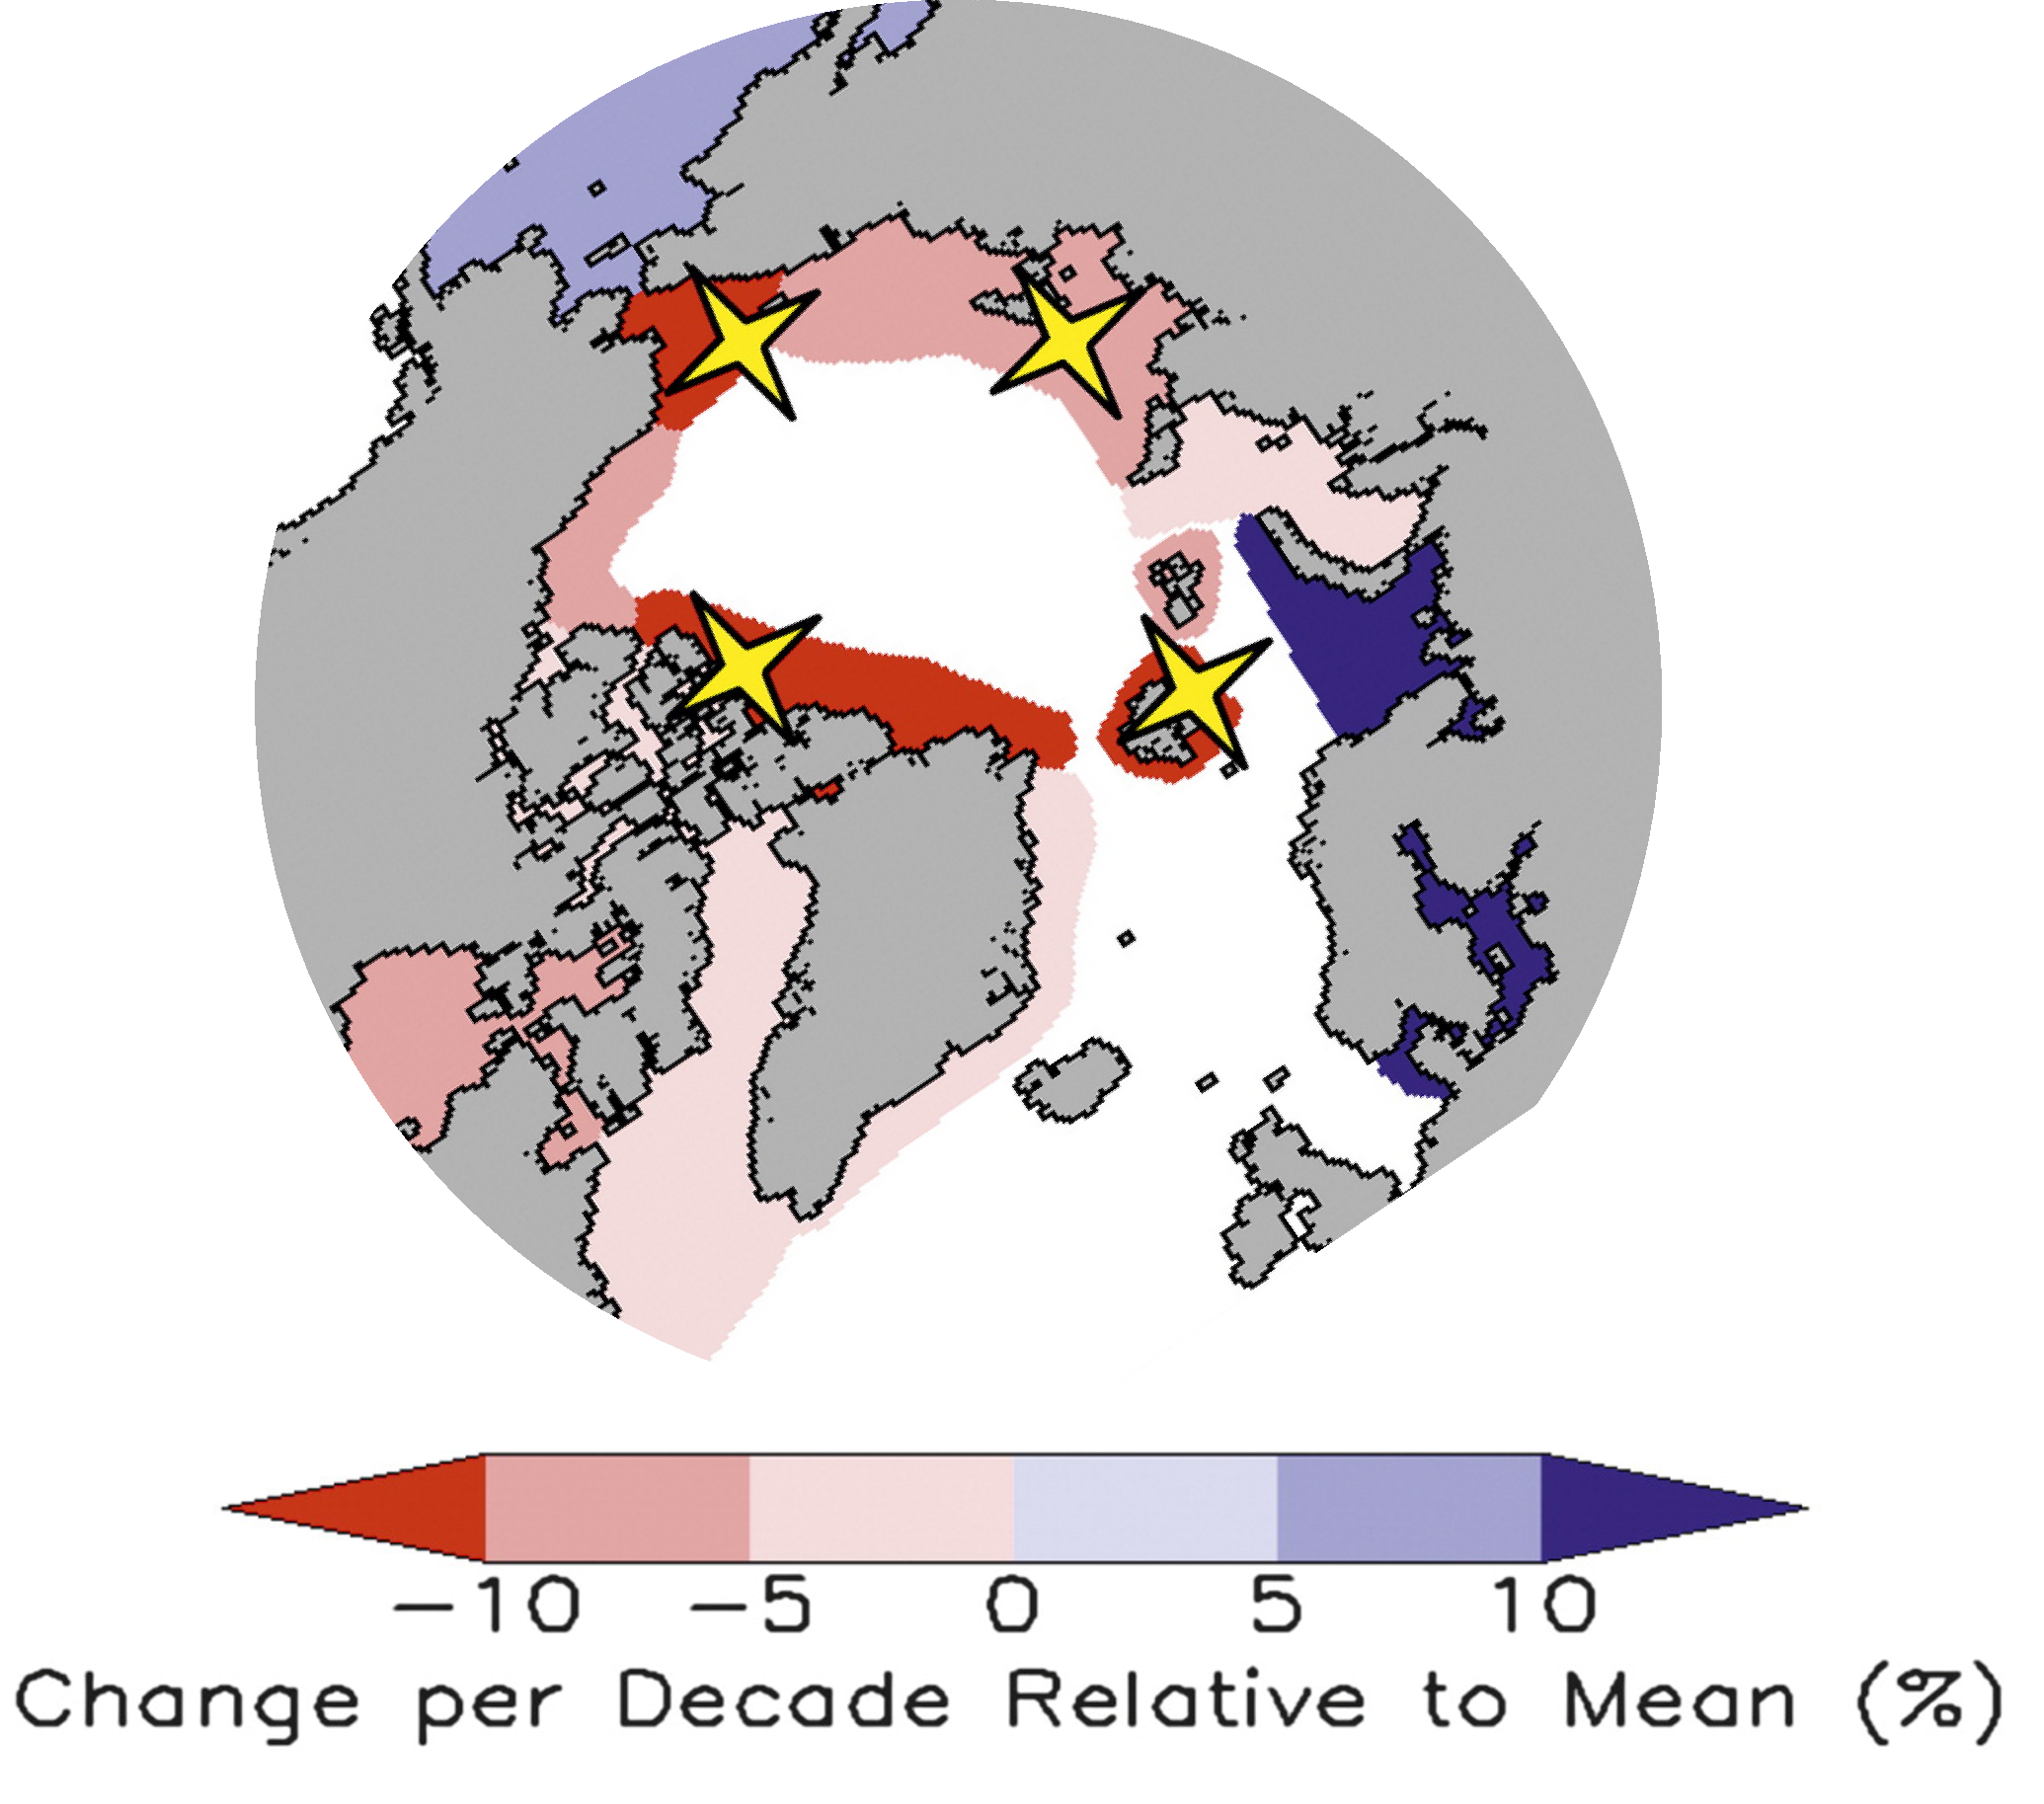
\includegraphics[width=0.8\textwidth]{./img/yu.pdf}\\\Fontvi
		(Yu et al.2014)
		\column{0.5\textwidth}
	
		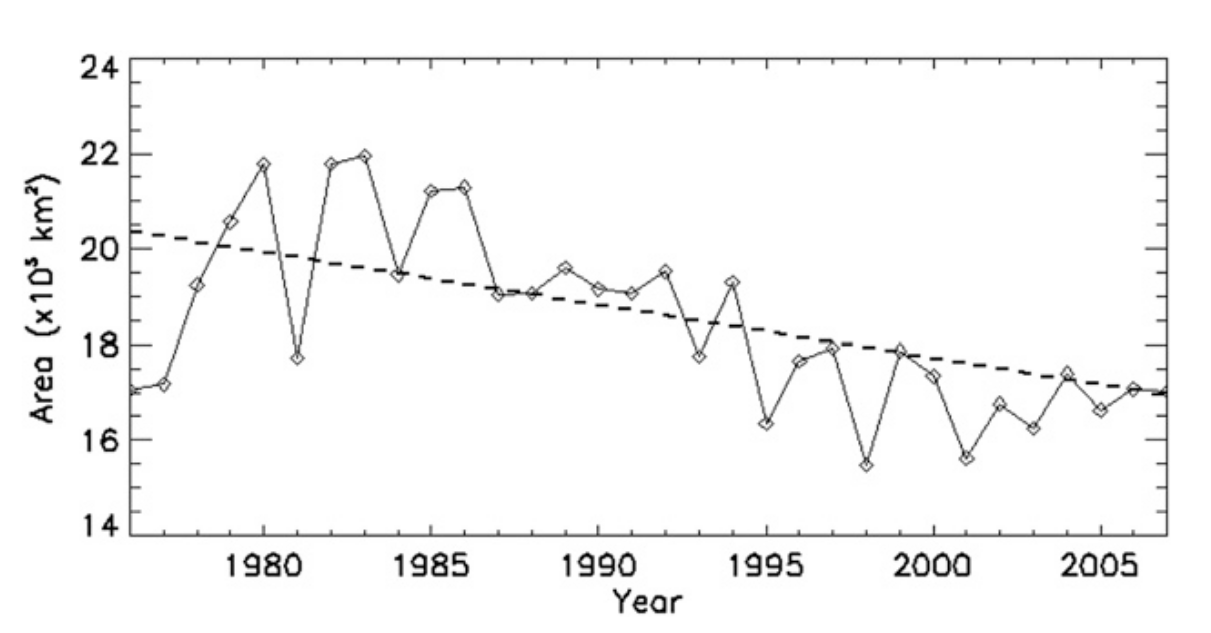
\includegraphics[width=0.8\textwidth]{./img/Extent_timeseries.png}\\
		\Fontvi
		(Yu et al.2014)
	\end{columns}
	\begin{columns}
		\column{0.25\textwidth}
		\column{0.5\textwidth}
	\begin{block}{\centering}
	\textbf{overall decrease in extent}\\
	LS - 8.4$\%$ per decade
	\end{block}
	\begin{block}{\centering}
	 \textbf{shorter landfast ice season}
	 LS - 2.5 weeks per decade
	 \end{block}
	 \column{0.25\textwidth}
	 \end{columns}

\end{frame}

%slide 9
\setwatermark{\fontsize{125pt}{125pt}\selectfont{}}
\begin{frame}[fragile]{I. Factors controlling variability of fast ice winter extent}
	\begin{center}
		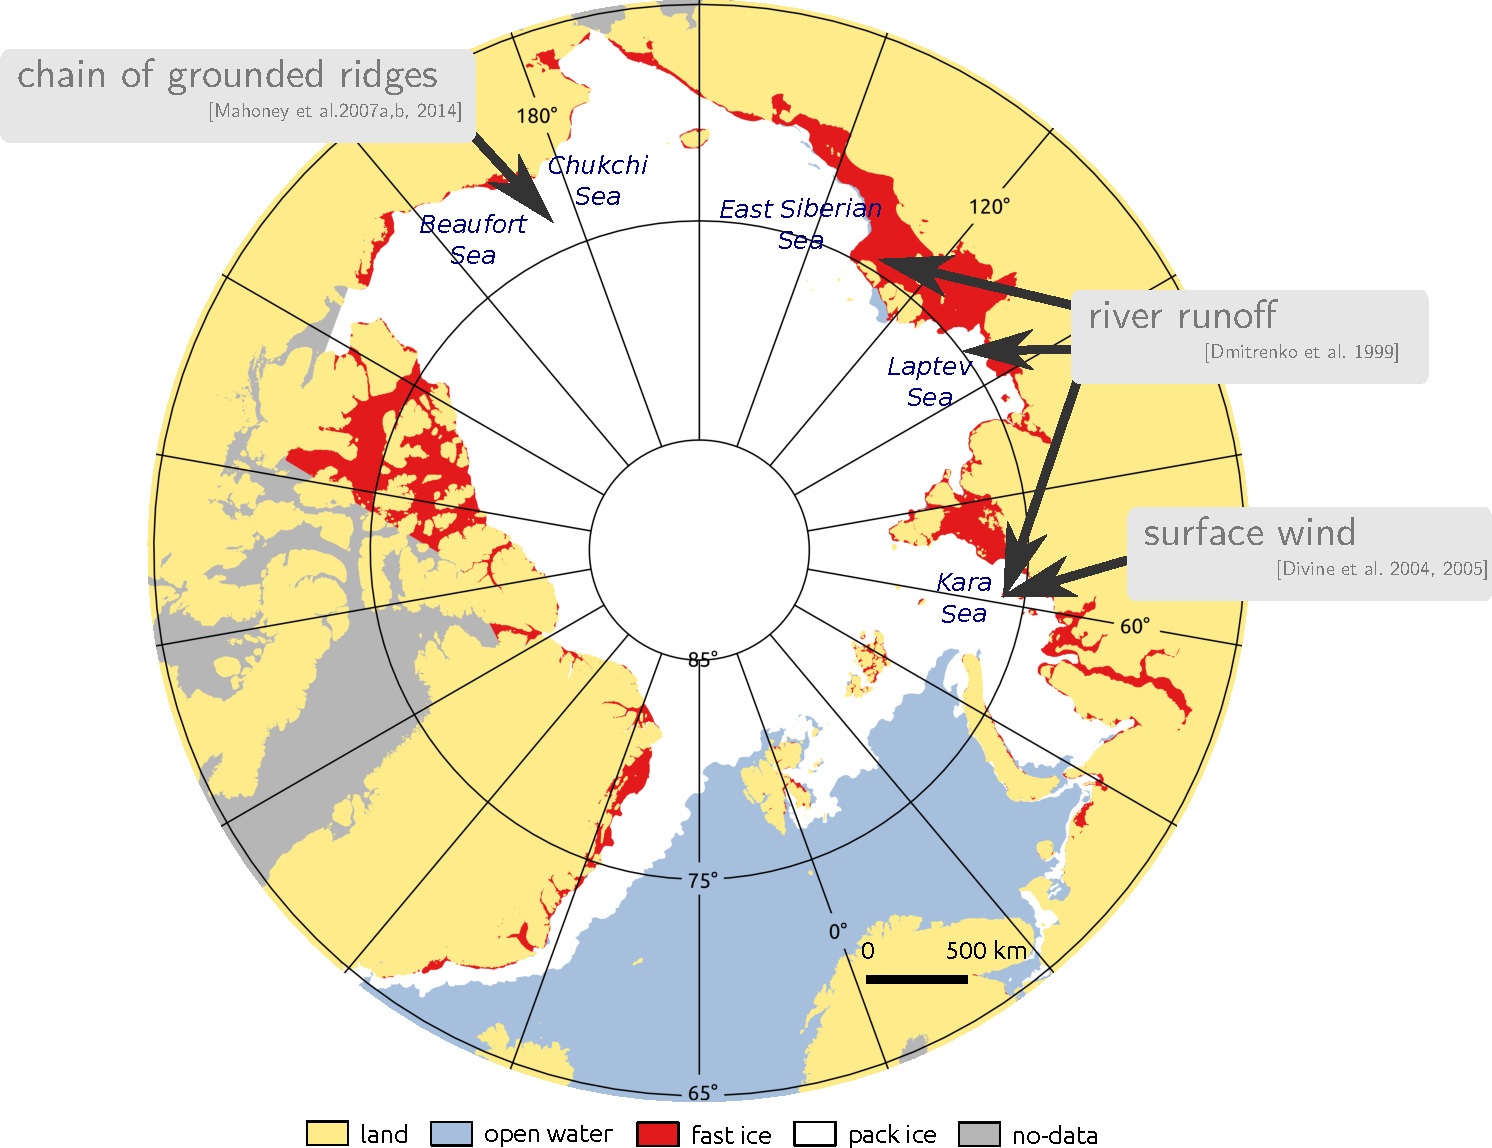
\includegraphics[height=7cm]{./img/ArcticSI_Mar2015_FI_know.pdf}\\
	\end{center}
	~\\
	\Fontvi
	17 March 2015 (AARI Charts)
\end{frame}

%slide 10
\setwatermark{\fontsize{125pt}{125pt}\selectfont{}}
\begin{frame}[fragile]{I.Objectives}
		
	Objective 1 -  Annual variability
		\begin{itemize}
			\item To describe the \textbf{annual fast ice cycle} and 
		reveal the \textbf{mechanisms driving the seasonal development} of fast ice.\\~\\
		\end{itemize}
	Objective 2 - Interannual variability and changes
		\begin{itemize}
			\item To evaluate \textbf{changes} in fast ice cover \textbf{on interannual scales} and 
		link them to climate processes.
		%\item higher domination of younger ice types\\~\\
		\end{itemize}

\end{frame}

%slide 11
\setwatermark{\fontsize{125pt}{125pt}\selectfont{}}
\begin{frame}[fragile]{II. Regions of interest and fast ice information}
	
	\begin{columns}
		\column{0.45\textwidth}
			\begin{center}
				Laptev Sea (LS)
				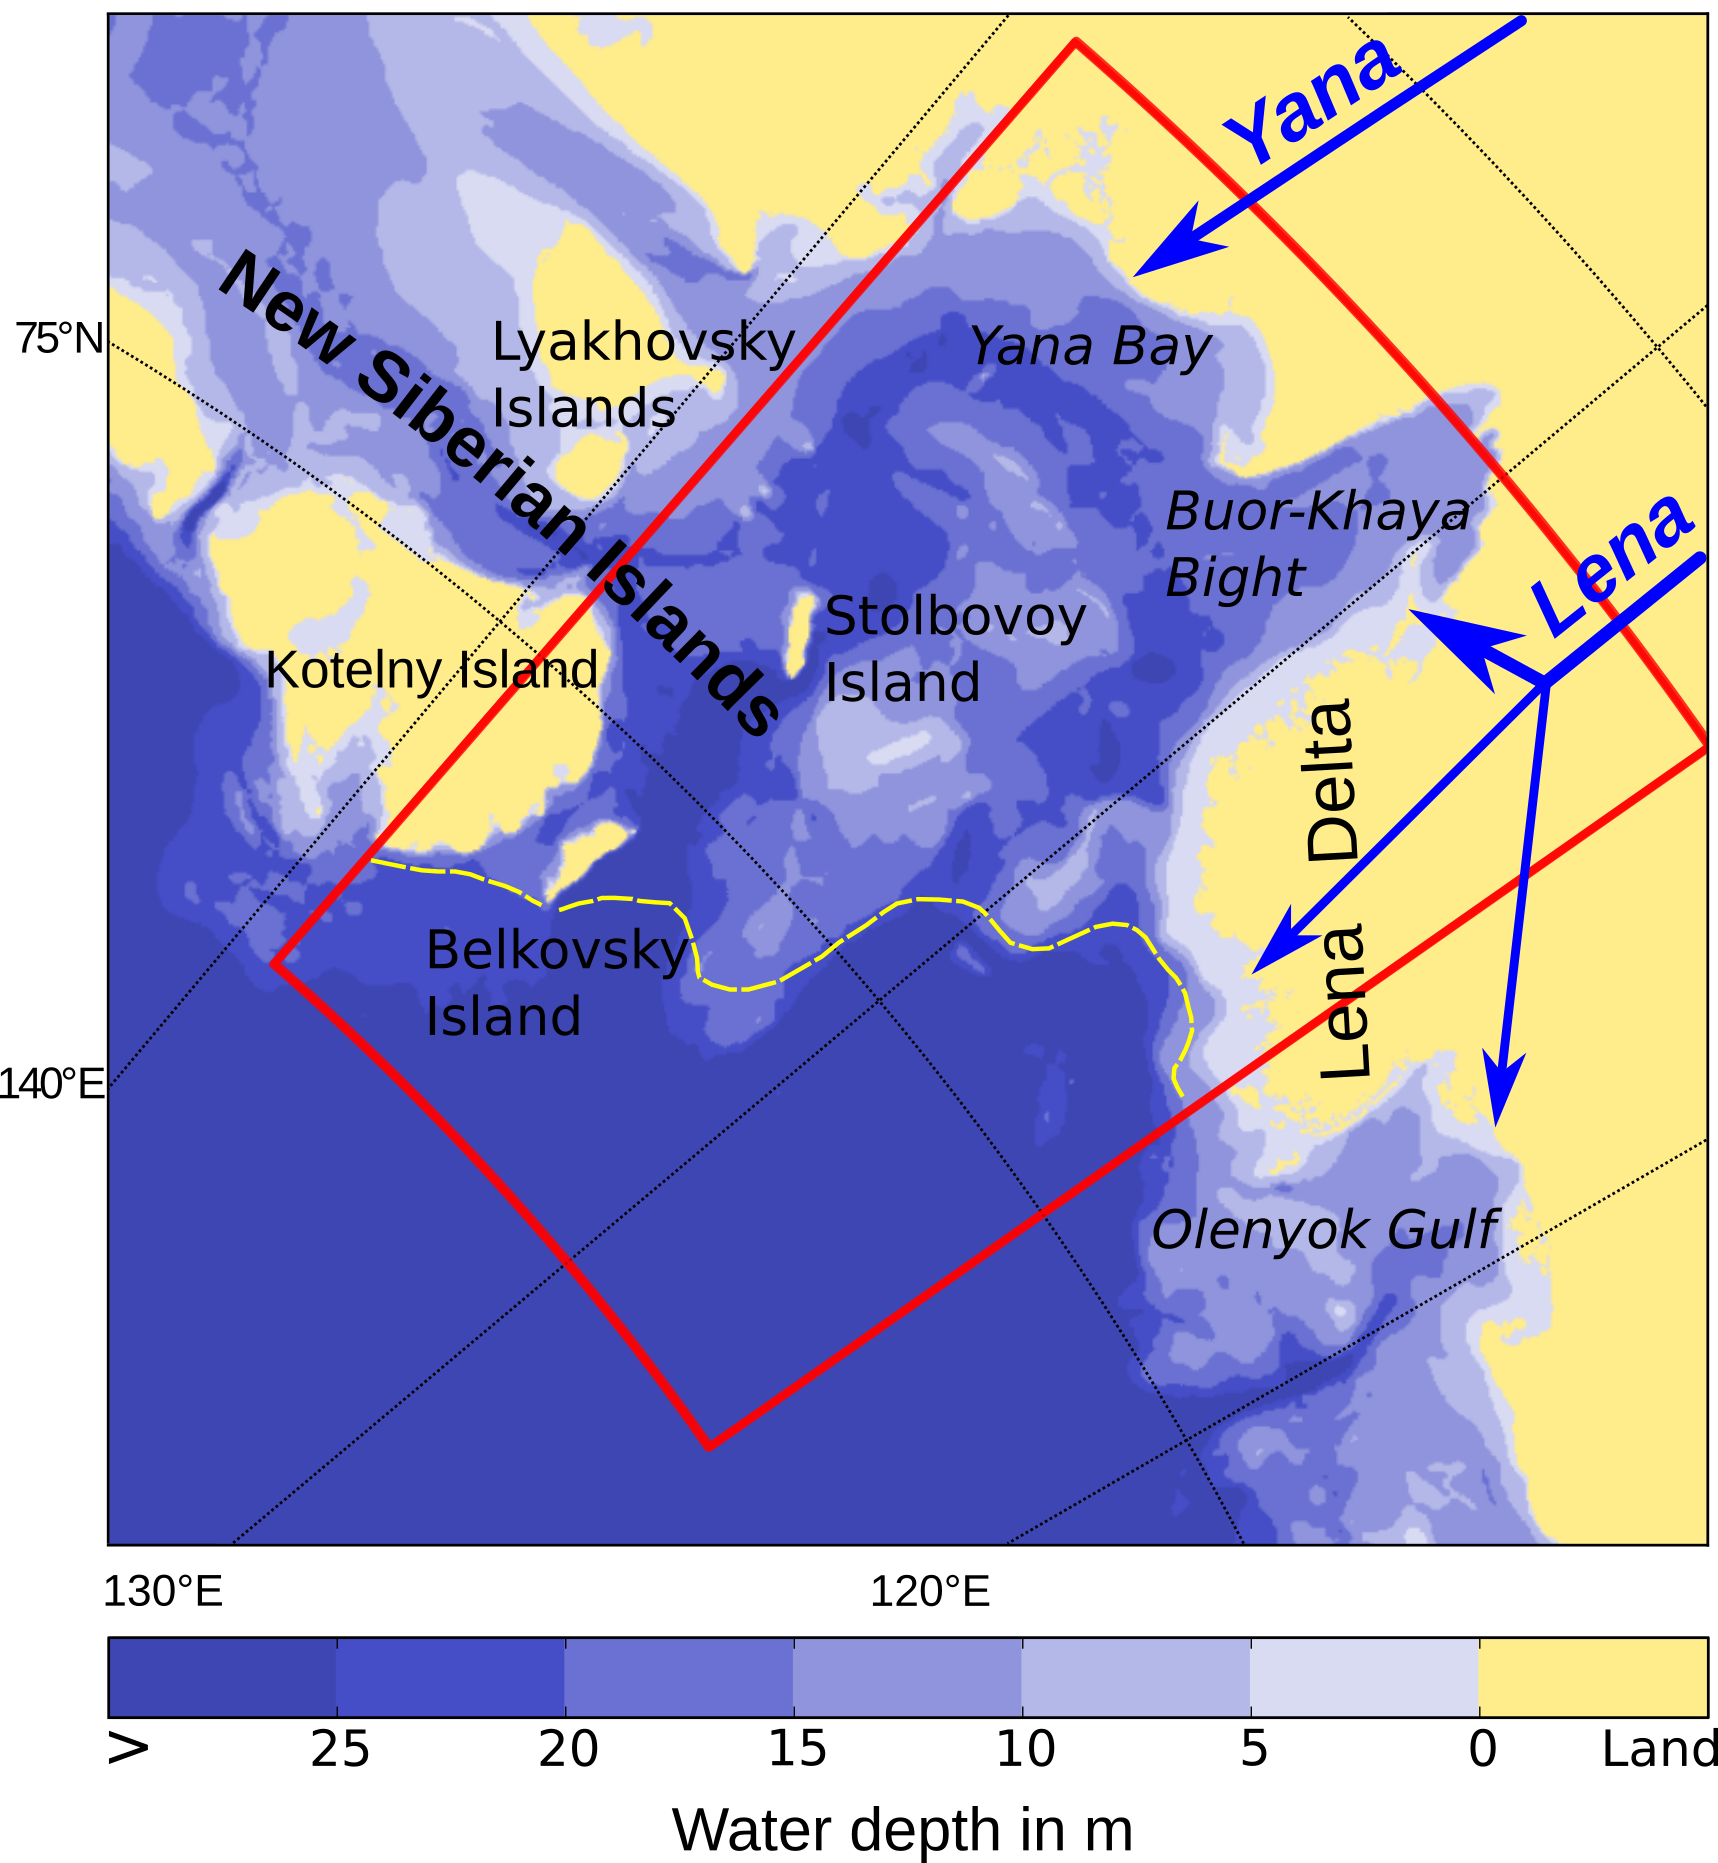
\includegraphics[height=5cm]{./img/LaptevBath.png}\\
				\textbf{AARI charts, 1999-2013, weekly}
			\end{center}
		\column{0.1\textwidth}
		\column{0.45\textwidth}
			\begin{center}
				East Siberian Sea (ESS)
				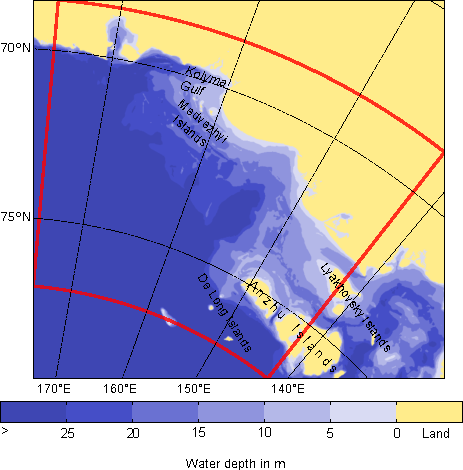
\includegraphics[height=5cm]{./img/ESSBath.pdf}\\
				\textbf{AARI charts, 1999-2013, weekly}
			\end{center}	
%			\begin{flushright}
%				\Fontvi
%				Selyuzhenok et al.(2015)
%			\end{flushright}
	\end{columns}
\end{frame}

%slide 12
\setwatermark{\fontsize{125pt}{125pt}\selectfont{}}
\begin{frame}[fragile]{II. Annual fast ice cycle, 2000-2001 }
	\begin{columns}
		\column{0.45\textwidth}
		\animategraphics[loop,autoplay,width=\linewidth]{3}{/home/valeria/Jacobs/Defense/defense/laptev/m-}{2}{41}
		\column{0.45\textwidth}
		\animategraphics[loop,autoplay,width=\linewidth]{3}{/home/valeria/Jacobs/Defense/defense/ESS/m-}{0}{39}
	\end{columns}
\end{frame}

%slide 13
\setwatermark{\fontsize{125pt}{125pt}\selectfont{}}
\begin{frame}[fragile]{II. Mean annual fast ice cycle}
	\begin{columns}
		\column{0.45\textwidth}
			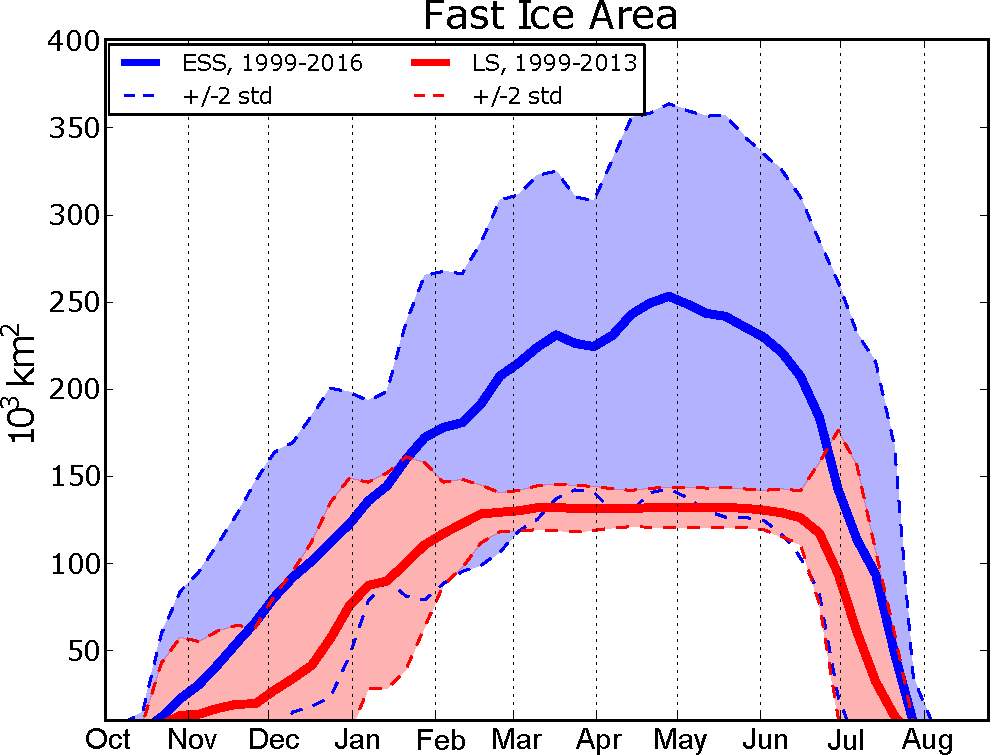
\includegraphics[height=6cm]{./img/Mean_SeasonalCycle_ESSvsSELS.pdf}\\
		\column{0.2\textwidth}
		\column{0.35\textwidth}
			\begin{center}
				\textbf{Interannual variability}\\~\\
				\textbf{Laptev Sea:}
			\end{center}
				\begin{itemize}
					\item high in November-February
					\item low throughout the rest of season
					\item the lowest in winter
			\end{itemize}
			
			\begin{center}
				\textbf{East Siberian Sea:}
				\begin{itemize}
					\item the highest  in winter
				\end{itemize}
			\end{center}
	\end{columns}
	
%	\begin{block}{\centering}
%		\begin{center}
%			ESS and LS landfast ice extents are controlled by different mechanisms
%		\end{center}
%	\end{block}
\end{frame}

%slide 14
\setwatermark{\fontsize{125pt}{125pt}\selectfont{}}
\begin{frame}[fragile]{II. Key events of annual cycle}
	\begin{columns}
		\column{0.60\textwidth}
		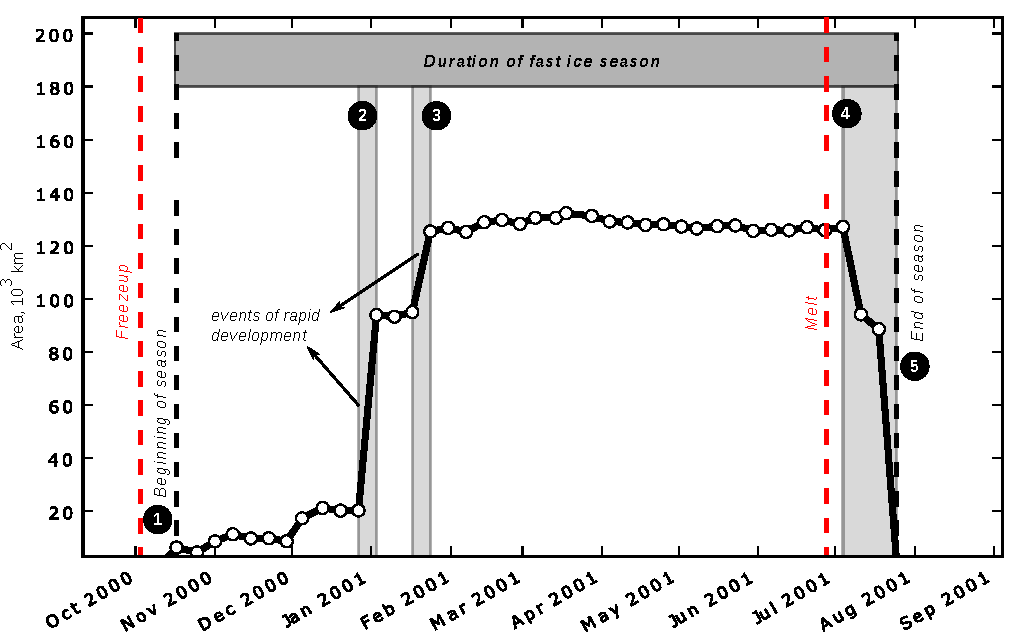
\includegraphics[width=1.0\textwidth]{./img/Key_events_LS0.pdf}\\~\\
	A typical annual fast ice cycle for the Laptev Sea
		\Fontvi
	(Selyuzhenok et al. 2015)
		\column{0.40\textwidth}
			\begin{center}
				\textbf{Laptev Sea,1999-2013 }\\~\\
				%\textbf{1999-2013}\\~\\
				Time series of Key events  1-5
			\end{center}
			~\\
			\begin{center}
				\textbf{East Siberian Sea, 1999-2015}\\~\\
				%\textbf{1999-2015}\\~\\
				Time series of Key events  1,5\\~\\ and Key events 2,3 for some seasons
			\end{center}
		\end{columns}
\end{frame}

%slide 15
\setwatermark{\fontsize{125pt}{125pt}\selectfont{}}
\begin{frame}[fragile]{II. Beginning of season}
	\begin{columns}
		\column{0.50\textwidth}
		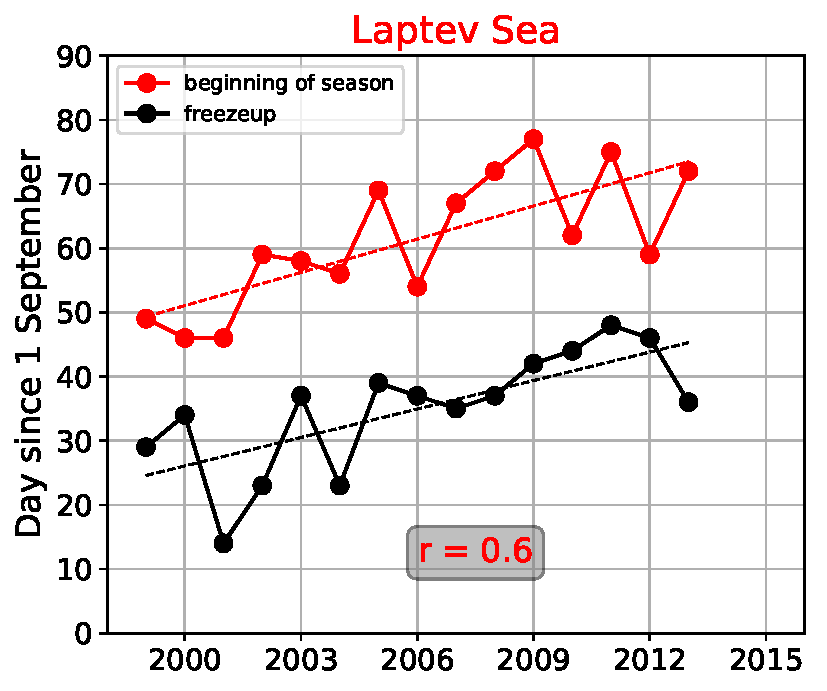
\includegraphics[width=0.9\textwidth]{./img/Beginning_frzp_LS.pdf}\\~\\
		\column{0.50\textwidth}
		\begin{itemize}
			\item{tendency towards later formation \\ 1.7 days/year (p\textless0.01)}\\~\\
			\item{partly explained by delay in freezeup\\ (r = 0.6)}
		\end{itemize}
	\end{columns}
\end{frame}

%slide 16
\setwatermark{\fontsize{125pt}{125pt}\selectfont{}}
\begin{frame}[fragile]{II. Rapid development}
	\begin{columns}
		\column{0.50\textwidth}
		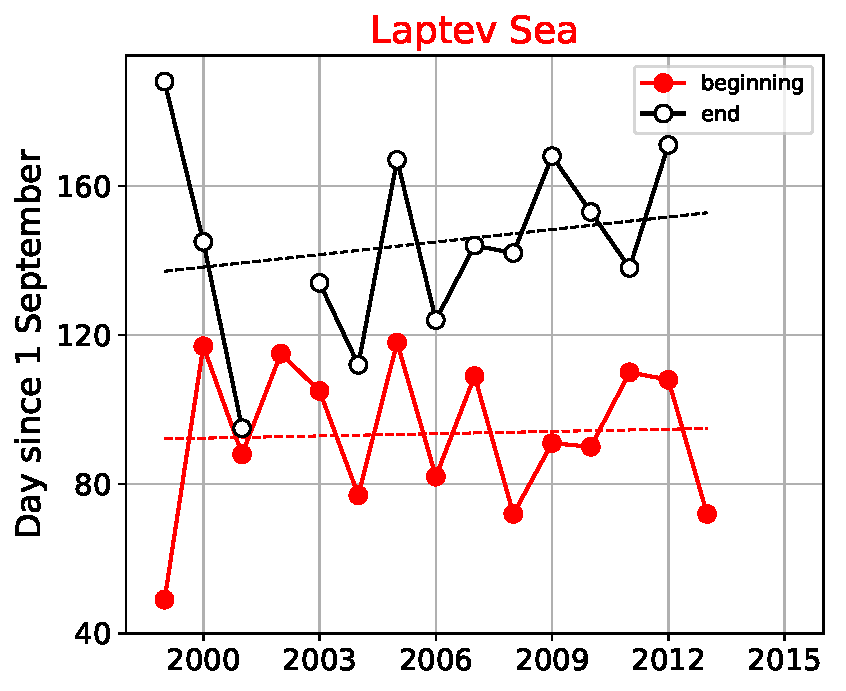
\includegraphics[width=0.9\textwidth]{./img/Rgrth_LS.pdf}\\~\\
		\column{0.50\textwidth}
		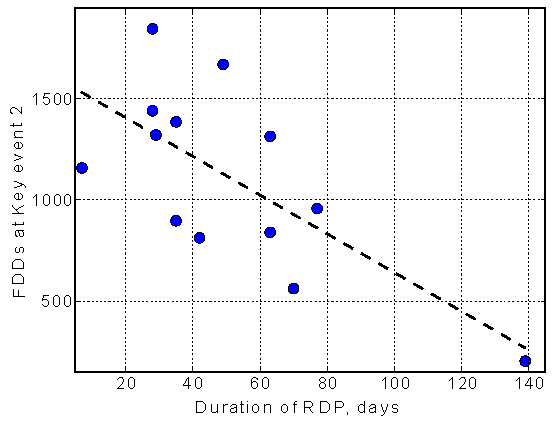
\includegraphics[width=0.9\textwidth]{./img/RGRTH_FDD.pdf}\\~\\
	\end{columns}
	
	\begin{columns}
		\column{0.50\textwidth}
		\begin{itemize}
			\item{high variability of dates}\\~\\
			\item{tendency towards later end \\ 0.4 days/year (p=0.07)\\}
		\end{itemize}
		\column{0.50\textwidth}
		\begin{itemize}
			\item{duration of period depends on\\ accumulated FDD}\\~\\
			\item{there is a critical ice thickness (Hi) required for rapid ice development\\ Hi(FDD) = 70-80 cm}
		\end{itemize}
	\end{columns}
\end{frame}

%slide 17
\setwatermark{\fontsize{125pt}{125pt}\selectfont{}}
\begin{frame}[fragile]{II. Breakup}
	\begin{columns}
		\column{0.50\textwidth}
		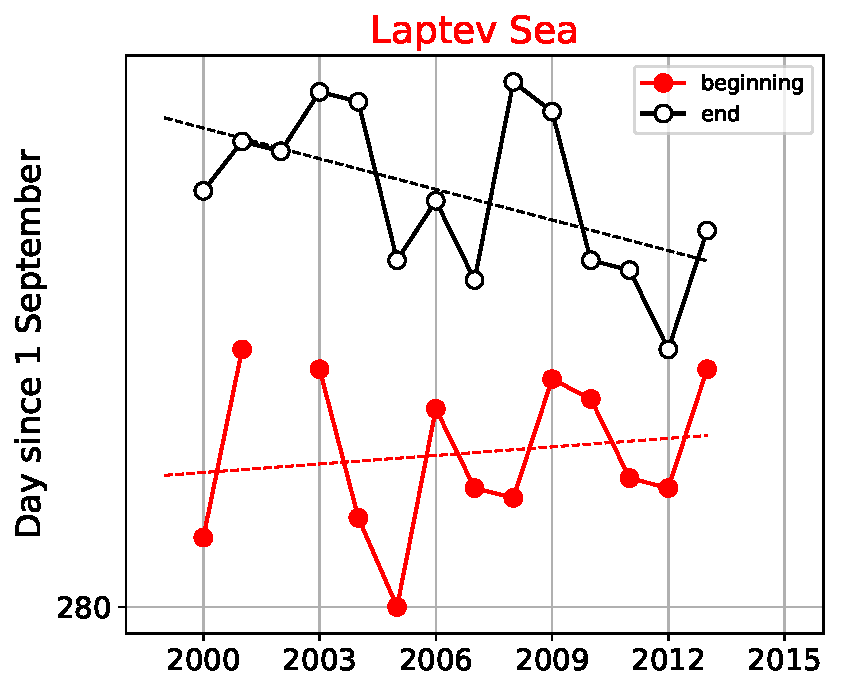
\includegraphics[width=0.9\textwidth]{./img/Brkp_LS.pdf}\\~\\
		\column{0.50\textwidth}
		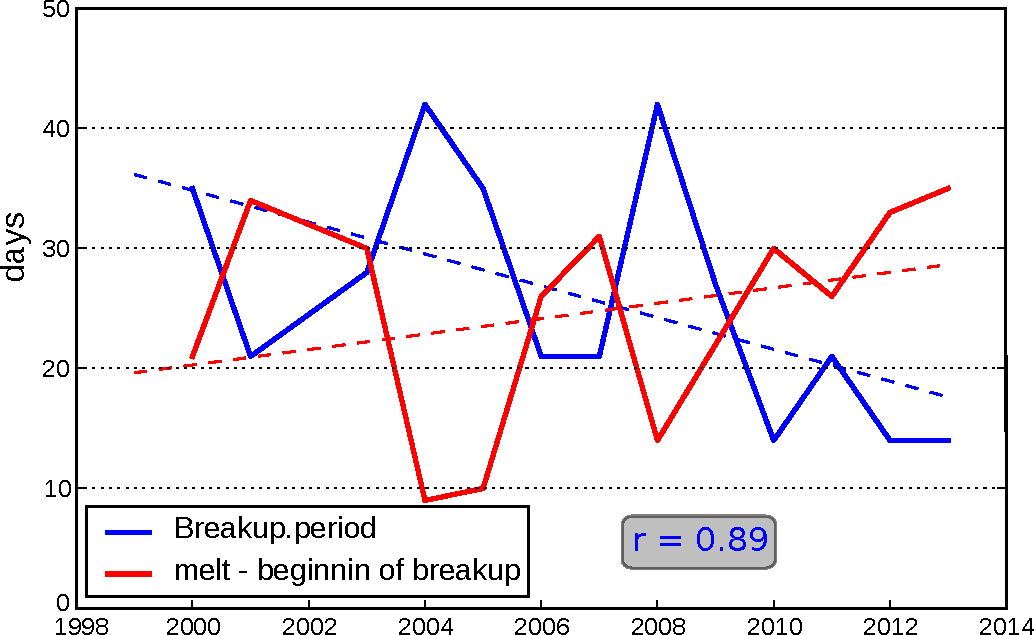
\includegraphics[width=0.9\textwidth]{./img/Breakup.pdf}\\~\\
	\end{columns}
	
	\begin{columns}
		\column{0.50\textwidth}
		\begin{itemize}
			\item{tendency towards earlier end\\ -1.0 days/year (p=0.06)}\\~\\
			\item{no changes in beginning \\ 0.3 days/year (p=0.63)\\}
		\end{itemize}
		\column{0.50\textwidth}
		\begin{itemize}
			\item{fast ice needs less time to breakup}\\~\\
			\item{duration of breakup depend on TDD acquired prior beginning of breakup }
		\end{itemize}
	\end{columns}
\end{frame}

%%%slide 17
%\setwatermark{\fontsize{125pt}{125pt}\selectfont{}}
%\begin{frame}[fragile]{II. Breakup}
%	\begin{columns}
%		\column{0.50\textwidth}
%		\centering
%%		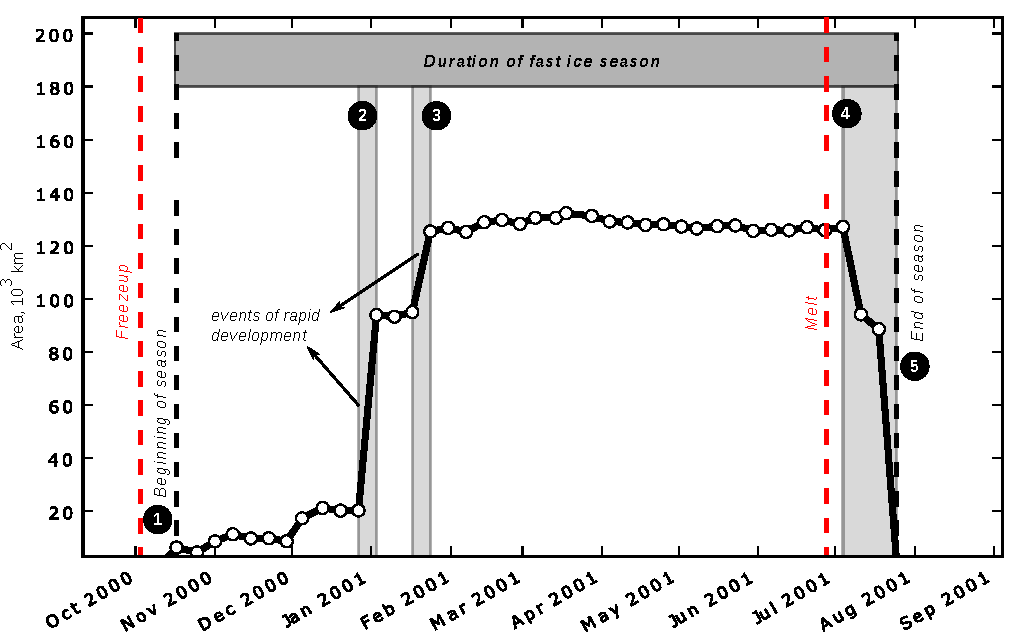
\includegraphics[width=1\textwidth]{./img/Key_events_LS0.pdf}
%		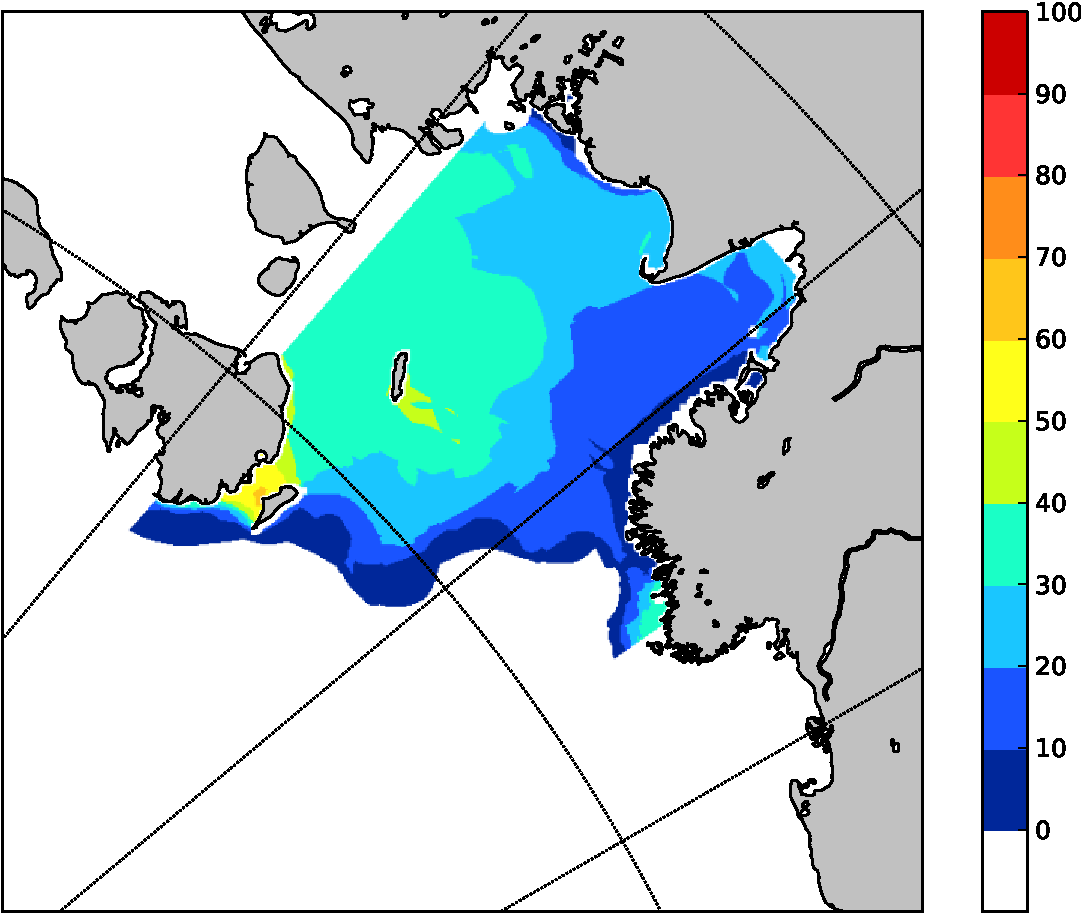
\includegraphics[width=0.8\textwidth]{./img/7_62_fr_av_clbr.pdf}
%		\column{0.50\textwidth}
%		\centering Duration of breakup
%		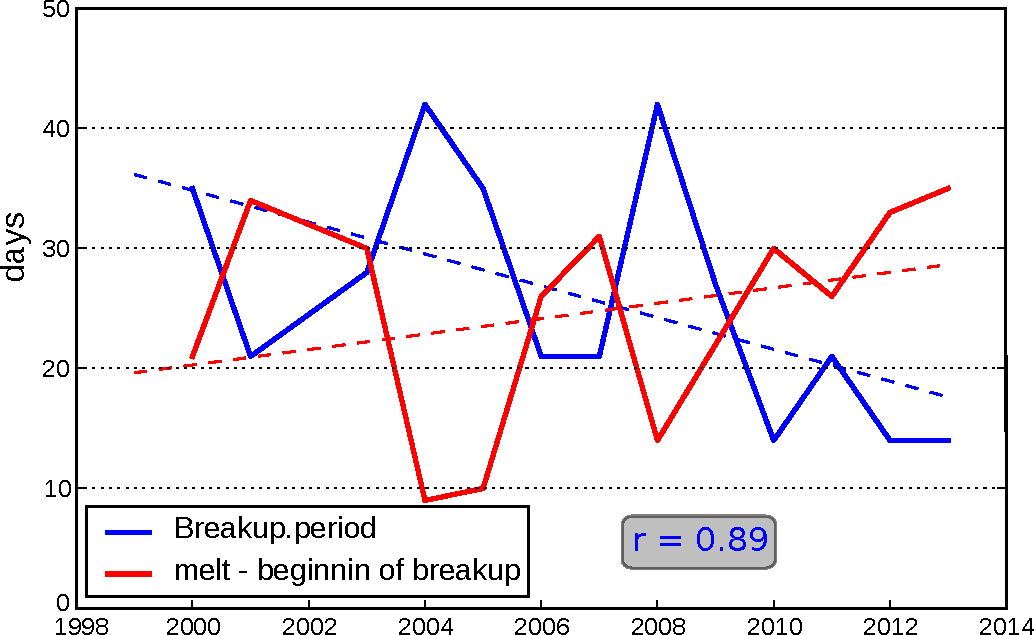
\includegraphics[width=1\textwidth]{./img/Breakup.pdf}
%		\begin{itemize}
%		\item fast ice needs less time to breakup
%		\item more time between melt onset and beginning of breakup --> shorter period of breakup
%		\end{itemize}
%	\end{columns}
%\end{frame}


%%slide 17
\setwatermark{\fontsize{125pt}{125pt}\selectfont{}}
\begin{frame}[fragile]{II.Winter landfast ice extent}
	\begin{columns}
		\column{0.70\textwidth}
		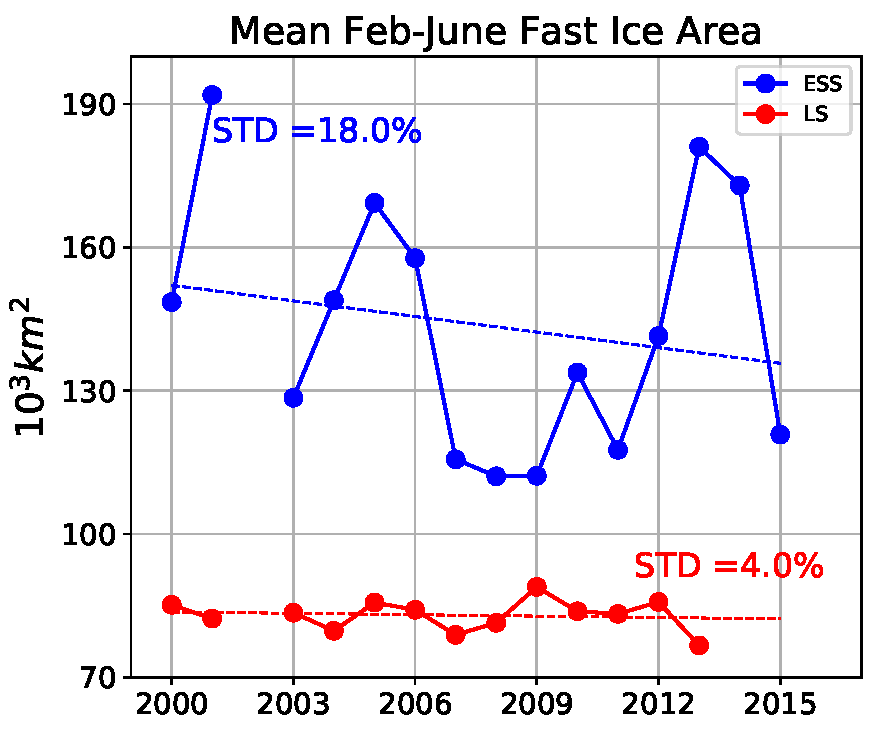
\includegraphics[width=1\textwidth]{./img/WinterArea_FebMay.pdf}
		\column{0.50\textwidth}
		\begin{itemize}
			\item no statistically significant changes in winter areal extent
		\end{itemize}
	\end{columns}
\end{frame}

%%slide 18
\setwatermark{\fontsize{125pt}{125pt}\selectfont{}}
\begin{frame}[fragile]{II. Annual variability and interannual changes}
\begin{columns}
	\column{0.50\textwidth}
	\centering
	\textbf{Laptev Sea}\\~\\
		\begin{itemize}
			\item high variation during fall development\\~\\
			\item later formation\\~\\
			\item shorter period of breakup\\~\\
			\item shorter fast ice season (by 2.8 days/decade)\\~\\
			\item no changes in winter extent\\~\\
		\end{itemize}
	
	\column{0.50\textwidth}
		\centering
	\textbf{East Siberian Sea}\\~\\
	\begin{itemize}
		\item high variability of winter extent\\~\\
		\item shorter fast ice season (by 1.5 day/year) 
	\end{itemize}
\end{columns}
\end{frame}

%%slide 19
\setwatermark{\fontsize{125pt}{125pt}\selectfont{}}
\begin{frame}[fragile]{II. Annual variability and interannual changes}
\begin{columns}
	\column{0.50\textwidth}
	\centering
	\textbf{Laptev Sea}\\~\\
	\begin{itemize}
		\item \textbf{high variation during fall development}\\~\\
		\item later formation\\~\\
		\item shorter period of breakup\\~\\
		\item shorter fast ice season (by 2.8 days/decade)\\~\\
		\item \textbf{no changes in winter extent}\\~\\
	\end{itemize}
	
	\column{0.50\textwidth}
	\centering
	\textbf{East Siberian Sea}\\~\\
	\begin{itemize}
		\item \textbf{high variability of winter extent}\\~\\
		\item shorter fast ice season (by 1.5 day/year) 
	\end{itemize}
\end{columns}
\end{frame}

%%slide 20
\setwatermark{\fontsize{125pt}{125pt}\selectfont{}}
\begin{frame}[fragile]{III.Laptev Sea : comparison of landfast ice information}
\begin{columns}
	\column{0.70\textwidth}
	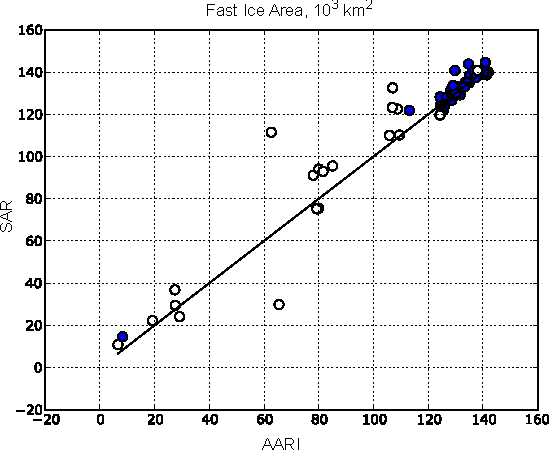
\includegraphics[width=1\textwidth]{./img/SAR_AARI.pdf}
	\column{0.50\textwidth}
	\begin{itemize}
		\item fast ice mapped by two experts 
		\item high deviations during development in fall
	\end{itemize}
\end{columns}
\end{frame}

%%slide 21
\setwatermark{\fontsize{125pt}{125pt}\selectfont{}}
\begin{frame}[fragile]{III.Laptev Sea : Case study of winter 2008/9 and 2009/10}
\begin{columns}
	\column{0.70\textwidth}
	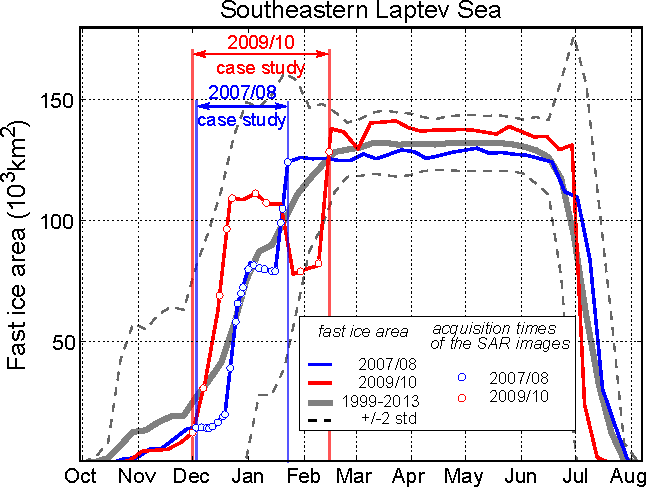
\includegraphics[width=1\textwidth]{./img/casestudy.pdf}
	\column{0.50\textwidth}
	\begin{itemize}
		\item SAR image every 2-14 days
		%\item fall fast ice extent is unambiguous  
	\end{itemize}
\end{columns}
\end{frame}

%%slide 22
\setwatermark{\fontsize{125pt}{125pt}\selectfont{}}
\begin{frame}[fragile]{III.Tracked sea ice features}

		\begin{center}
		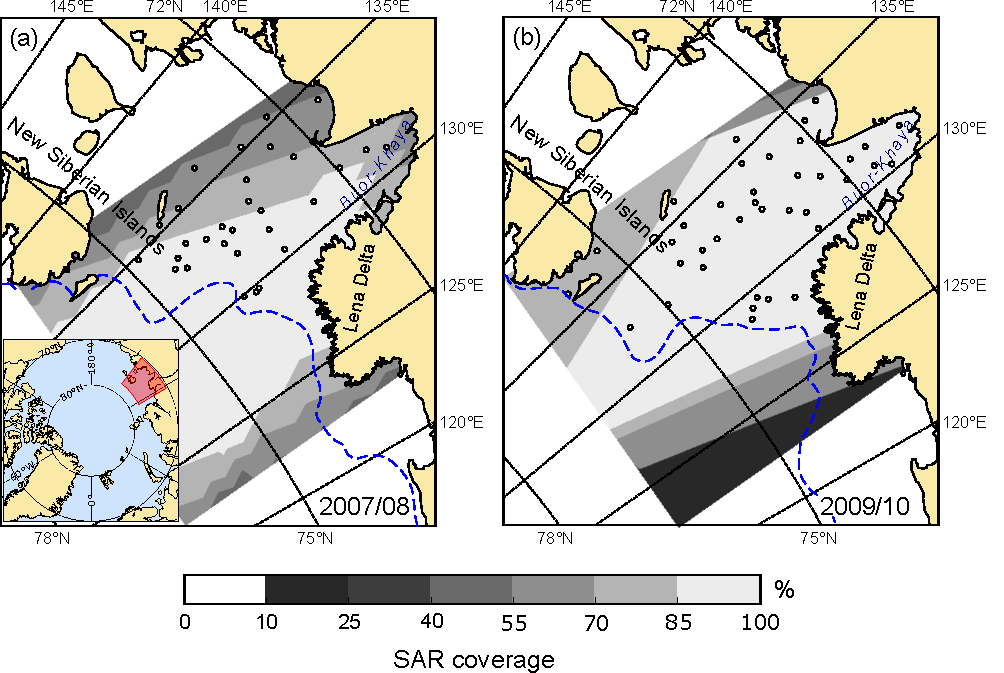
\includegraphics[width=0.9\textwidth]{./img/trackpoints.pdf}\\
		fast ice =  drift speed \textless 0 cm/s
		\end{center}

\end{frame}

%%slide 23
\setwatermark{\fontsize{125pt}{125pt}\selectfont{}}
\begin{frame}[fragile]{III. Patterns of drift}
	\begin{center}
			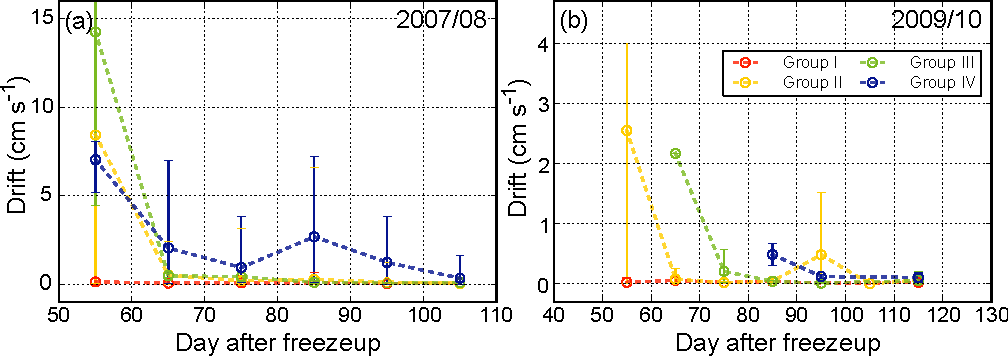
\includegraphics[width=0.8\textwidth]{./img/groups_graph.pdf}\\~\\
			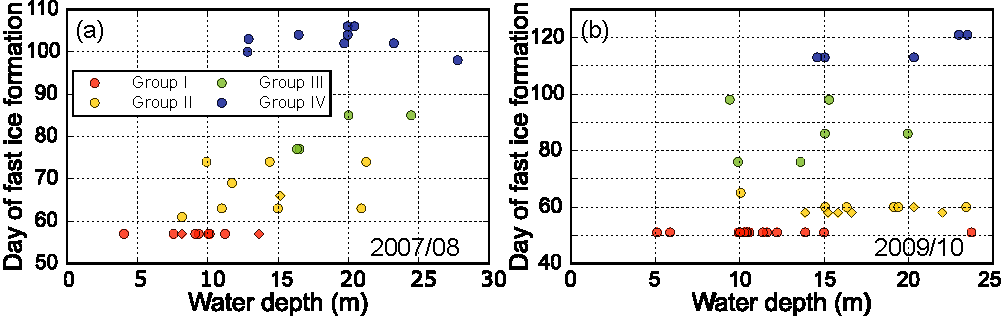
\includegraphics[width=0.8\textwidth]{./img/groups_depth.pdf}
	\end{center}
\end{frame}

%%slide 25
\setwatermark{\fontsize{125pt}{125pt}\selectfont{}}
\begin{frame}[fragile]{III. Final location of features}
\begin{center}
	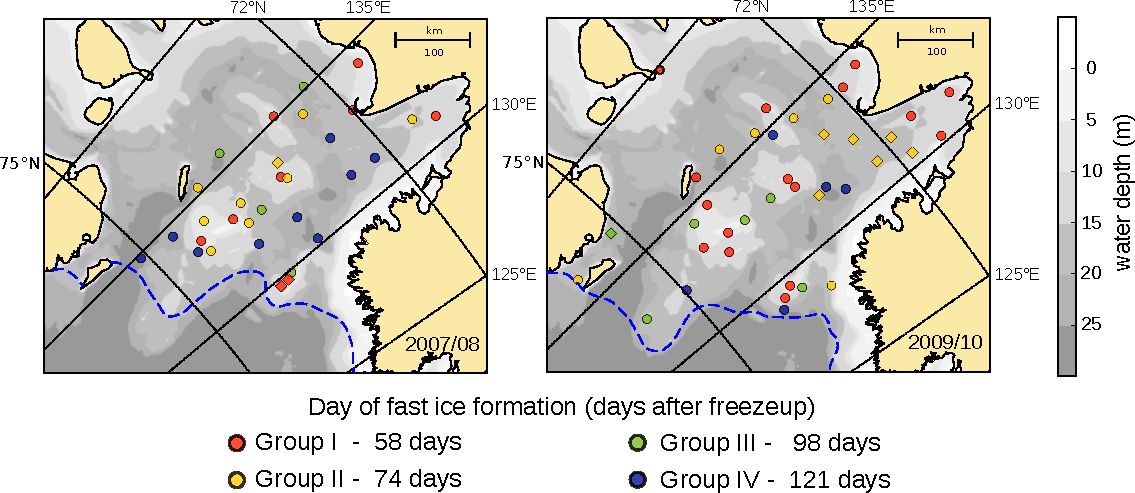
\includegraphics[width=0.9\textwidth]{./img/groups_map.pdf}
\begin{itemize}
\item relatively thin ice becomes grounded over the shoals (red circles)\\
\item it serves as stabilizing points for surrounding sea ice
\item low variations in winter extent predefined by the bathymetry
\end{itemize}
\end{center}
\end{frame}

%%slide 25
\setwatermark{\fontsize{125pt}{125pt}\selectfont{}}
\begin{frame}[fragile]{III.Deep sea ice ridges}
\begin{columns}
	\column{0.40\textwidth}
	End of Rapid Development
		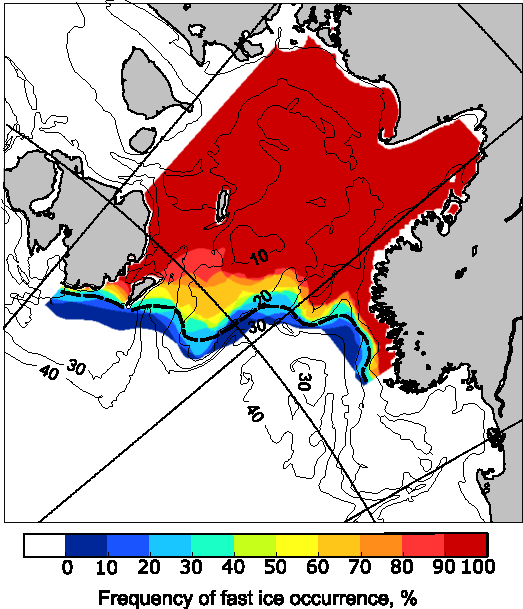
\includegraphics[width=0.9\textwidth]{./img/Rgrth_freqency.pdf}
	\column{0.60\textwidth}
		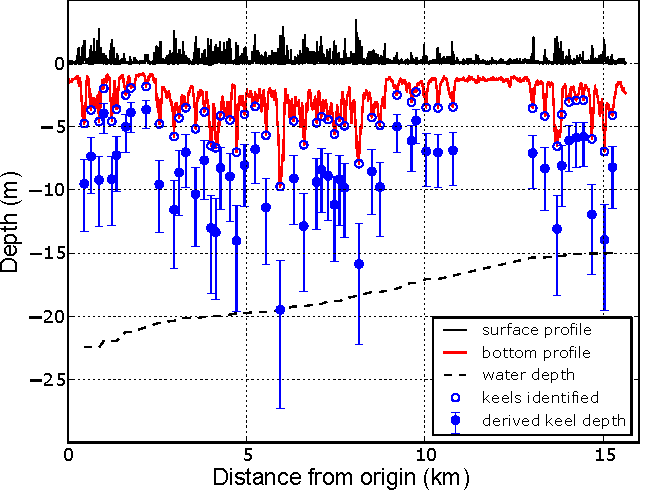
\includegraphics[width=0.9\textwidth]{./img/EM_profile.pdf}
	\end{columns}
\begin{itemize}
	\item variations in winter fast ice edge is likely controlled by grounding of deep ice ridges
\end{itemize}
\end{frame}

%%slide 26
\setwatermark{\fontsize{125pt}{125pt}\selectfont{}}
\begin{frame}[fragile]{III.East Siberian Sea Fast ice modes}
\begin{center}
	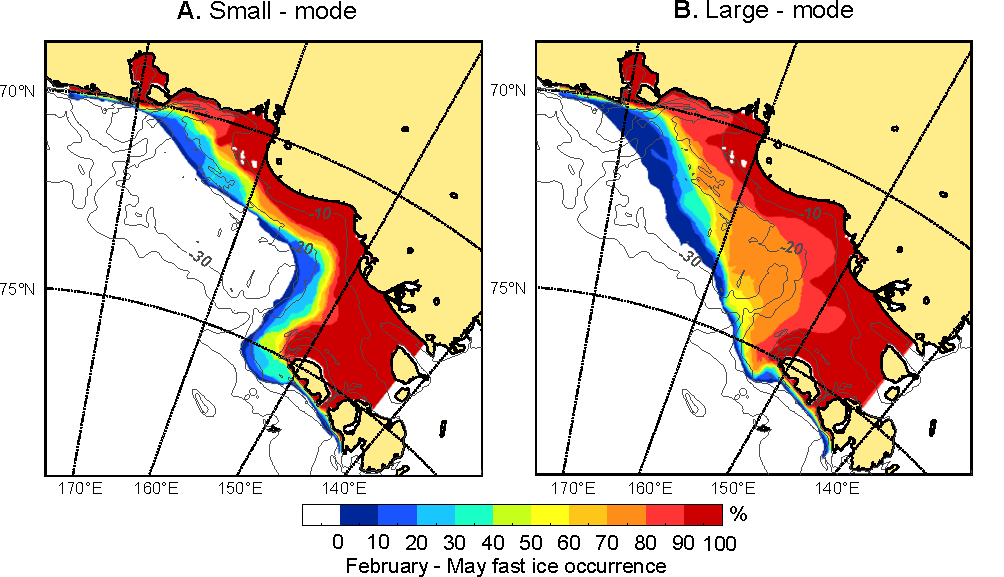
\includegraphics[width=0.9\textwidth]{./img/ESS_modes.pdf}
%	\begin{itemize}
%		\item relatively thin ice becomes grounded over the shoals (red circles)\\
%		\item it serves as stabilizing points for surrounding sea ice
%		\item low variations in winter extent predefined by the bathymetry
%	\end{itemize}
\end{center}
\end{frame}

%%slide 28
\setwatermark{\fontsize{125pt}{125pt}\selectfont{}}
\begin{frame}[fragile]{III. Arctic Oscillation index}
	\begin{columns}
		\column{0.50\textwidth}
		Positive Arctic Oscillation index (AO)
		\includegraphics[width=0.9\textwidth]{./img/LowAO_Rigor.PNG}

		\column{0.50\textwidth}
		Negative Arctic Oscillation index (AO)	\includegraphics[width=0.9\textwidth]{./img/HighAO_Rigor.PNG}
	%	\begin{itemize}
	%		\item relatively thin ice becomes grounded over the shoals (red circles)\\
	%		\item it serves as stabilizing points for surrounding sea ice
	%		\item low variations in winter extent predefined by the bathymetry
	%	\end{itemize}
\end{columns}
\end{frame}

%%slide 29
\setwatermark{\fontsize{125pt}{125pt}\selectfont{}}
\begin{frame}[fragile]{III.East Siberian Sea fast ice modes}
\begin{center}
\begin{columns}
	\column{0.70\textwidth}
	\centering
	February-May AO and fast ice modes
	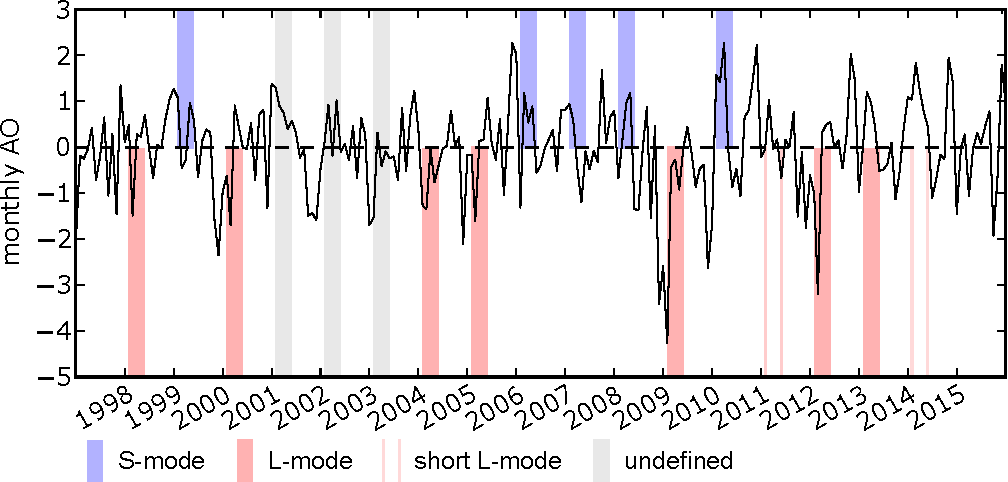
\includegraphics[width=1\textwidth]{./img/AO.pdf}\\~\\
	\begin{block}{Hypothesis}
		Sea ice import during AO+ leads to formation thick ice ridges, which become grounded and stabilize fast ice in L-mode.
	\end{block}
	\column{0.3\textwidth}
	Negative AO
	%\includegraphics[width=0.7\textwidth]{./img/HighAO_Rigor.png}\\~\\
	\includegraphics[width=0.7\textwidth]{/home/valeria/Jacobs/Defense/defense/img/HighAO_Rigor.PNG}\\~\\
	Positive AO
	%\includegraphics[width=0.7\textwidth]{./img/LowAO_Rigor.png}
	\includegraphics[width=0.7\textwidth]{/home/valeria/Jacobs/Defense/defense/img/LowAO_Rigor.PNG}
\end{columns}	

%\begin{itemize}
%	\item import of thick ice/increased deformation during +AO periods 
%	\item thick ridges become grounded over deeper water
%	\item grounded ridges stabilize fast ice in L-mode
%\end{itemize}

\end{center}
\end{frame}

%slide 2
\setwatermark{\fontsize{125pt}{125pt}\selectfont{}}
\begin{frame}{Summary}
	\begin{block}{Objective 1 -  Annual variability}
		\begin{itemize}
			\item Annual fast ice cycle described with Key events
			\item Sea ice grounding is a key process in annual fast ice development
		\end{itemize}
	\end{block}
	\begin{block}{Objective 2 - Interannual variability and changes}
		\begin{itemize}
			\item Tendency towards shorter fast ice season (LS - 2,8 days/year, ESS - 1.5 days/year)
			\item No changes in winter fast ice extent
			\item Shorter time required for fast ice to breakup in summer 
		\end{itemize}
	\end{block}
\end{frame}

%%slide 2
%\setwatermark{\fontsize{125pt}{125pt}\selectfont{}}
%\begin{frame}{Outlook}
%\begin{block}{Objective 1 -  Annual variability}
%	\begin{itemize}
%		\item Annual fast ice cycle described with Key events
%		\item Sea ice grounding is a key process in annual fast ice development
%	\end{itemize}
%\end{block}
%\begin{block}{Objective 2 - Interannual variability and changes}
%	\begin{itemize}
%		\item Tendency towards shorter fast ice season (LS - 2,8 days/year, ESS - 1.5 days/year)
%		\item No changes in winter fast ice extent
%		\item Shorter time required for fast ice to breakup in summer 
%	\end{itemize}
%\end{block}
%\end{frame}
\end{document}